\documentclass{article}

\usepackage[fontsize=12.0pt]{fontsize}
\usepackage{times}
\usepackage[T1]{fontenc}
\usepackage[square,sort,comma,numbers]{natbib}
\bibliographystyle{abbrvnat}

\usepackage[margin=0.8in]{geometry}
\setlength{\parskip}{5pt}%

\setlength{\parindent}{0pt}
\usepackage[compact]{titlesec}

\usepackage{enumitem}
\usepackage{url}

\usepackage{mathtools, amsmath, amssymb, commath, fixmath}

\usepackage{titling}

\makeatletter
  \newcommand\tinyv{\@setfontsize\tinyv{12pt}{12}}
\makeatother

\usepackage{lipsum, wrapfig}
\usepackage{graphicx}
\graphicspath{{images/}}

%----------------------------------------------------------------------------------------
\begin{document}

\begin{flushleft}
\textbf{Course Title: CPSC545 - Algorithms in Bioinformatics} \\
Name: Yi Jou (Ruby) Liao, liao.yj.ruby@gmail.com \\
Name: Maxwell Douglas, mdouglas@bccrc.ca \\
\today
\end{flushleft}

\begin{center}
  \Large\textbf{Exploring Spatially Aware Dimensionality Reduction for Domain Detection in Spatial Transcriptomics}
\end{center}

\section*{Abstract}

Spatial transcriptomics has emerged as a contemporary analytical approach that facilitates the integration single cell RNA-seq data with spatial cellular positions. Our study investigates the influence of dimensionality reduction methods on cell clustering, aiming to leverage embedded spatial information for enhanced computational tissue structure interrogation. In response to the limited availability of challenging biological contexts in conventional benchmarking datasets, we simulate a glandular tissue structure to evaluate the effectiveness of domain detection with spatially aware dimensional reduction through SpatialPCA. Subsequently, we integrate SpatialPCA into the Seurat analysis pipeline within a ovarian cancer spatial transcriptomics study to assess the added value of spatially aware dimensionality reduction and its potential impact on uncovering biological insights.

\section*{Introduction}

Spatial transcriptomics, deemed “Method of the Year'' for 2020 by \textit{Nature Methods}\citep{marx2021}, allows for the collection of RNA-seq data along with the positional context of cells. Many spatial sequencing technologies are currently available and are able to capture information at a variety of cellular resolutions. Widely adopted, next generation sequencing based methods such as 10x Visium and Slide-seq\citep{rodriques_slideseq_2019} capture between 1-10 cells per bar-coded spot on a tissue slide. Single-cell resolution spatial transcriptomics is performed via in-situ RNA sequencing, and sub-cellular resolution can be achieved through methods based on single-molecular fluorescence in-situ hybridization (smFISH)\citep{williams_introduction_2022}. Experiments utilizing this technology, especially with integration of parallel single cell RNA-seq data, have led to new insights in areas such as cancer tumor structure\citep{lyubetskaya2022}, cellular interactions\citep{cang2023}, and development of cell atlases\citep{cui2023}.

A key step in downstream analysis of spatial transcriptomics data involves unsupervised clustering of similar spots or cells, where dimensionality reduction is commonly employed to enhance biological signals before applying a clustering algorithm. Over varied biologic structures, the detection of these biologically relevant clusters or collections of clusters is called 'domain-detection'. One of the major anticipated advantages of spatial transcriptomics is that because cell-neighbourhood information is embedded within the data-set, it will be easier to interrogate tissue structure computationally. To investigate that idea, our study looks at the impact of a dimensionality reduction method that integrates spatial information into cell-clustering.

Most current state of the art method studies doing domain detection in spatial transcriptomics test against a large number of common spatial data-sets such as DLPFC\citep{maynard_transcriptomescale_2021}, HER2 breast cancer\citep{wu_stromal_2020}, and their own simulated data-sets (SpatialPCA\citep{shang2022}, SRTsim\citep{zhu_srtsim_2023}, GIOTTO\citep{dries_giotto_2021}). This is an excellent practice for encouraging reproducibility and robustness in the computational biology literature. However, we have noticed that very rarely do these test data-sets include `harder' biological contexts. For example, the DLPFC data-set has 7 distinct tissue domains all stacked on top of one another. These tissue domains are separated by cells with well-known expression and functional differences. All of the recent methods we have seen successfully separate these tissue domains with little issue. So at this point, resolving tissue domains of that nature should be considered a baseline.

More difficult biological contexts are of interest because they speak to the ability of novel computational methods to assist in discovering new biology. Unfortunately, due to the recentness of the invention of Spatial Transcriptomics, this technique has not yet been widely adopted. Therefore, there is a paucity of quality data-sets easily accessible over the web. So what is the best next solution? Simulating these data-sets. In our study detailed below we chose to try and simulate more homogeneous tissue with less regular structure. In order to simulate the structure of glandular tissue we employed a newly developed R package called SRTsim (Spatially Resolved Transcriptomics simulations).

One of the central questions guiding the second part of our investigation was, how much utility or additional insight could be gained by applying spatially aware dimensional reduction to a typical research project applying spatial transcriptomics? Recent publications in the field, emphasizing translational applications of spatial transcriptomics for deriving biological insights rather than the development of bioinformatics algorithms, commonly rely on established analysis pipelines such as Seurat's\citep{hao2021} suggested workflow. Widely adopted analysis tools like Seurat, however, tend to not incorporate cutting edge spatial domain detection methods that may better exploit the embedded spatial information in spatial transcriptomics sequencing.

In order to investigate the potential impact of adopting a spatial analysis innovation such as spatially aware dimensional reduction on biological conclusions, we incorporated the SpatialPCA R package into a recently published case study paper that employed the standard Seurat spatial transcriptomics analysis pipeline that performs standard principal components analysis and compared downstream results.

\section*{Results}

\subsection*{Simulation benchmarking}

We used SRTsim to build an approximation of the structure of glandular tissue (see ground truth panel of Figure \ref{fig:simclustplot}). We simulated 4 different layers with a single protruding branch. Some obvious improvements are immediately evident with this test scenario (multi-branch structures, inward protrusions etc.) but due to time-constraints we felt this was an acceptable first step. Clear opportunities for expansions and future work will be outlined in the Discussion section. 

\begin{figure}[h!]
    \centering
    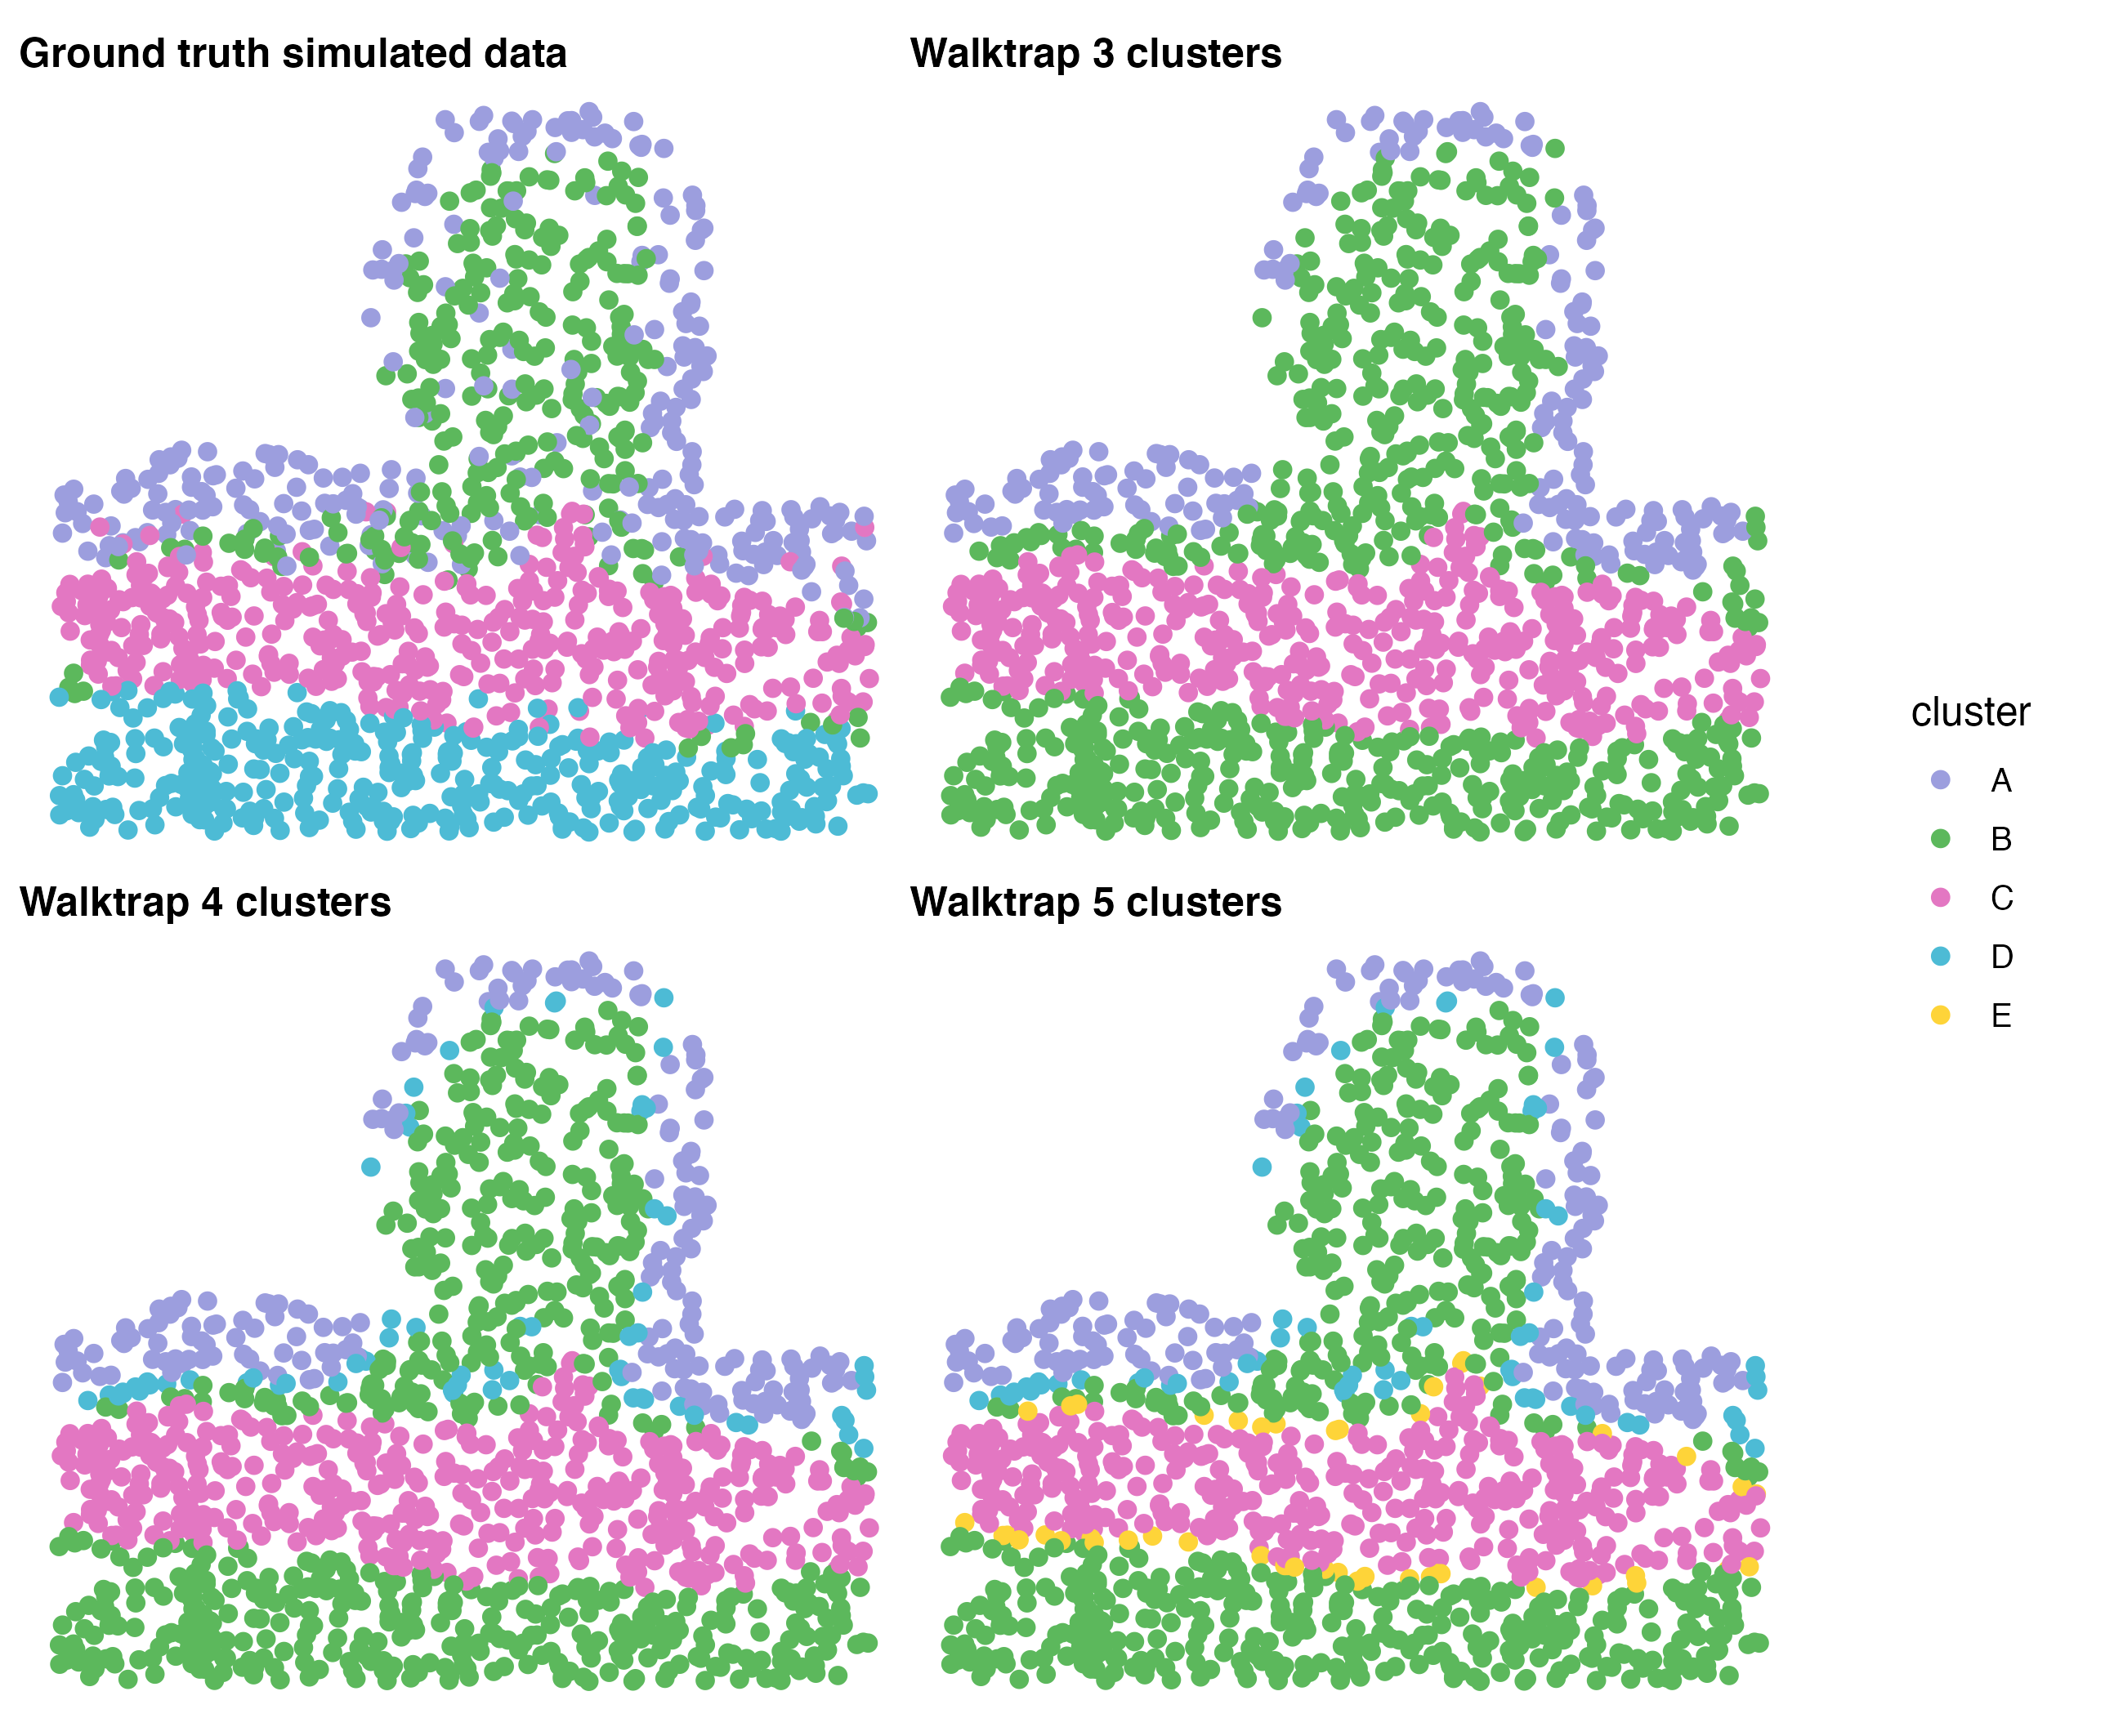
\includegraphics[width=0.75\textwidth]{images/clusters_plot.png}
    \caption{Simulated glandular test data-set coloured by clusters/domains. The ground truth domains are compared to those predicted after SpatialPCA and walktrap clustering.}
    \label{fig:simclustplot}
\end{figure}

The spatial domains detected using SpatialPCA and Walktrap clustering do not faithfully recapitulate the ground truth domains. This is clearly visible in the Walktrap panels of Figure \ref{fig:simclustplot}. While the majority of cells are separated in accordance with the true glandular structure there are two main departures: first, domains B and D in the ground truth data-set are universally detected as the same domain, and second, the borders between domains are instead treated as domains all their own. 

Analysis of average silhouette widths in Table \ref{tbl:sil_tbl} indicate a likely explanation for the results: the ground truth domains do not necessarily display a substantial difference in within-group similarity versus out-group similarity for clusters B and D. Silhouette width values close to +1 indicate well-clustered cells that are appropriately separated from neighboring clusters, while values around 0 suggest overlapping clusters, and values close to -1 indicates potential misclassifications or incorrect clustering.

\begin{table}[h!]
    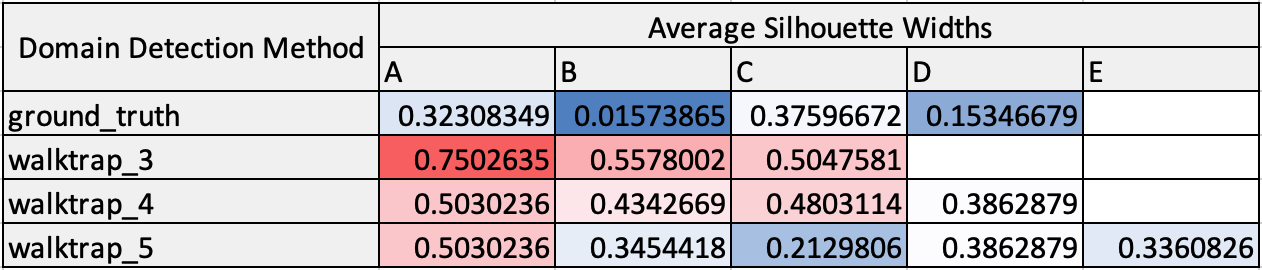
\includegraphics[width=\textwidth]{images/silhouette.png}
    \caption{Mean Silhouette widths. Silhouette widths were calculated per cluster/domain for each Walktrap run and for the ground truth domains.}
    \label{tbl:sil_tbl}
\end{table}

Moreover, the evaluation using CHAOS (Cluster Hierarchy and Order Scores) scores (Table \ref{tbl:chaos}) indicate that universally, the domains (true and predicted) are quite continuous, ordered, and may have a less-complex transcriptomic landscape. CHAOS is a metric used to assess the orderliness within clustering results, where scores closer to 0 indicate less structured clusters and scores closer to 1 suggest a more organized spatial arrangement of cells. The CHAOS score for the ground truth domain is close to 0 and the resulting Walktrap clustering CHAOS scores are of similar magnitude. 

\begin{table}[h!]
    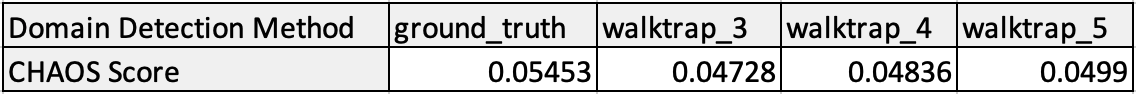
\includegraphics[width=\textwidth]{images/chaos.png}
    \caption{CHAOS Scores. A CHAOS score was calculated for each Walktrap run and for the ground truth domains.}
    \label{tbl:chaos}
\end{table}

Complementing the other clustering metrics, the LISI (Local Inverse Simpson's Index) scores as visualized in Figure \ref{fig:lisiplot} provide insight by emphasizing the transitions between domains. The lowest LISI score possible is 1, indicating accurate clustering where a cell's neighborhood only contains one cell type which is its own. As evident in the ``walktrap\_5\_clusters" panel, the cell spots located in the transitions between domains have the highest LISI score, indicating higher LISI scores, poorer clustering, and less defined domains in those regions.

\begin{figure}[h!]
    \centering
    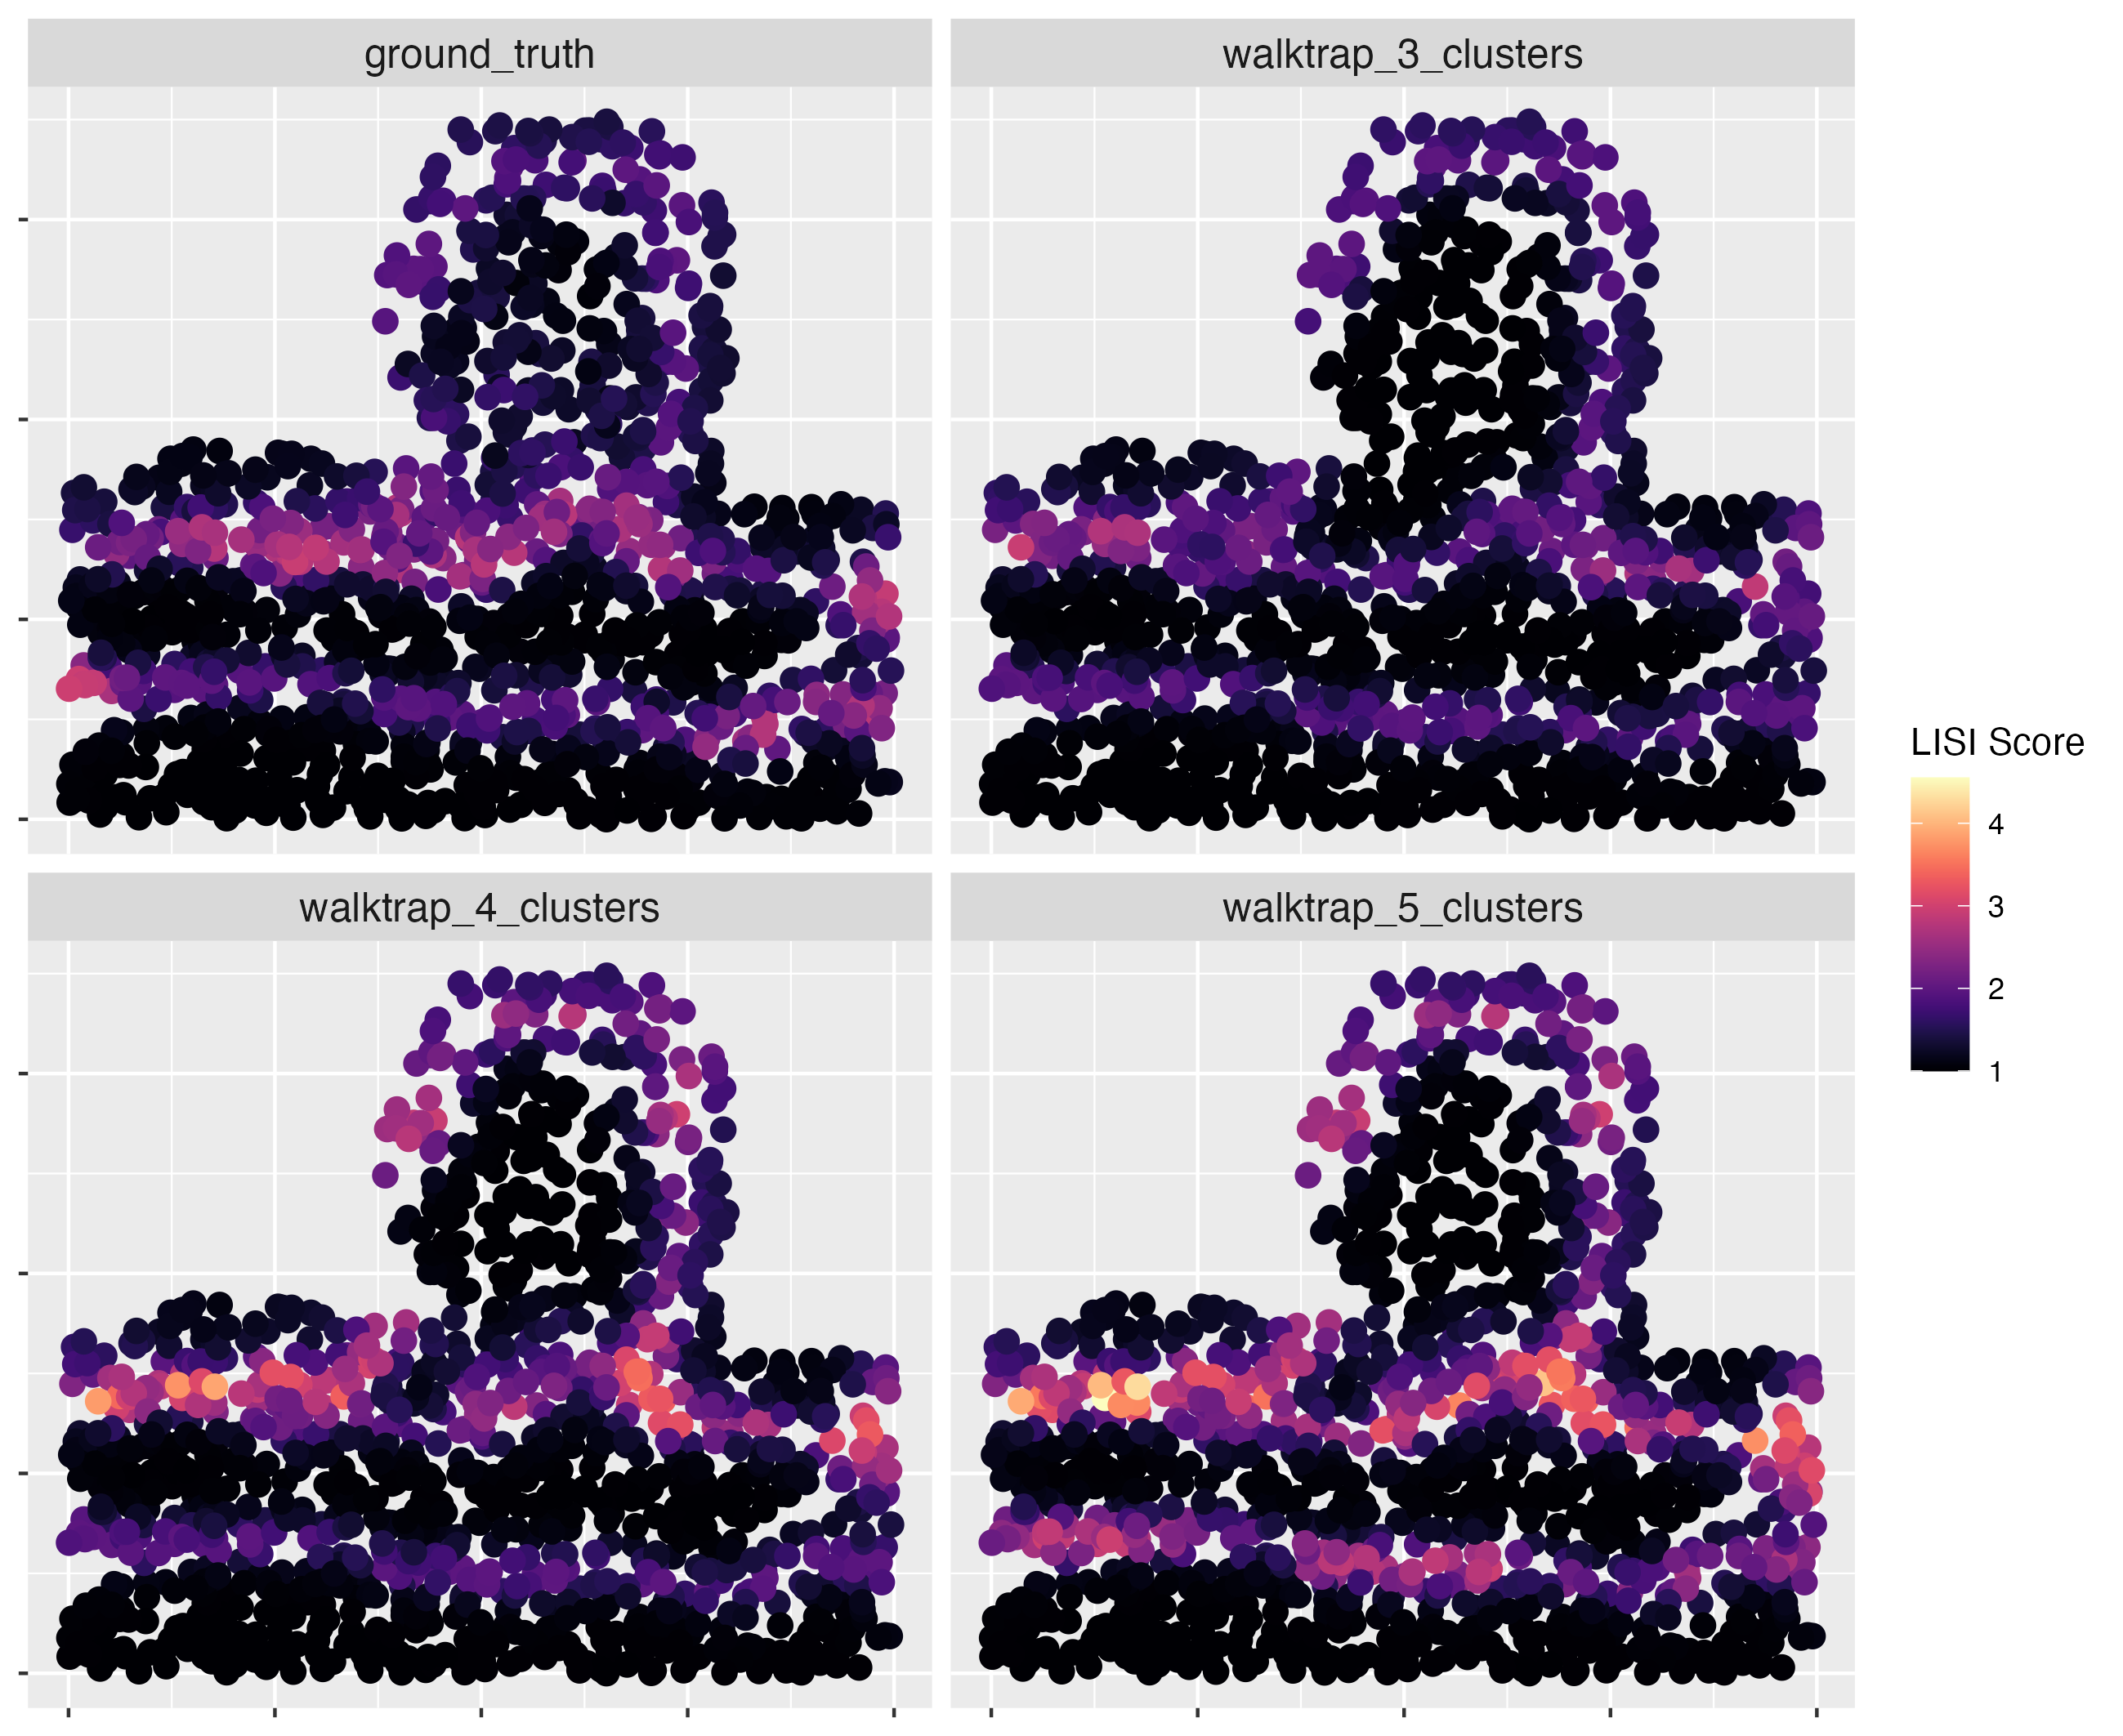
\includegraphics[width=0.75\textwidth]{images/LISI_plot.png}
    \caption{Simulated glandular test data-set coloured by LISI score. The ground truth domains are compared to those detected after SpatialPCA and walktrap clustering. A higher score means less smooth and continuous clusters/domains while a lower scores means the opposite.}
    \label{fig:lisiplot}
\end{figure}

\subsection*{Application to ovarian cancer spatial transcriptomics analysis}

To explore the impact and potential downstream analysis implications, we incorporated spatially aware dimensional reduction to the \citet{sanders_small_2022} paper reviewing a small cell carcinoma of the ovary hypercalcemic type (SCCOHT) case study. The first part describes a clinical patient case of SCCOHT, a rare and aggressive ovarian cancer type, in a patient with \textit{SMARCA4} and \textit{BRCA2} germline mutations. Guided by the genetic testing results as well as the rarity of this tumour type, they chose to apply spatial transcriptomics to further understand transcriptional heterogeneity in their case study. As seen in Fig. \ref{fig:Sanders_tissuefig}, the \citet{sanders_small_2022} analysis and interpretation primarily focused on sample `D-GTFB1170', where the 2495 capture spot were grouped into 12 distinct clusters according to transcriptional profiles. For the remainder of the results, we mainly focused on replicating and extending the spatial transcriptomics analysis for `D-GTFB1170' to be able to compare and contrast biological conclusions as presented in the paper.

Cluster cell types, as seen in the UMAP grouped by cluster plot in Fig. \ref{fig:Sanders_tissuefig}, were annotated based on Cell Type Signature gene sets as applied through gene set enrichment analysis (GSEA). Through the spatial transcriptomics analysis, they concluded that three clusters were associated with angiogenesis and endothelial cell biology.

\begin{figure}[h!]
    \centering
    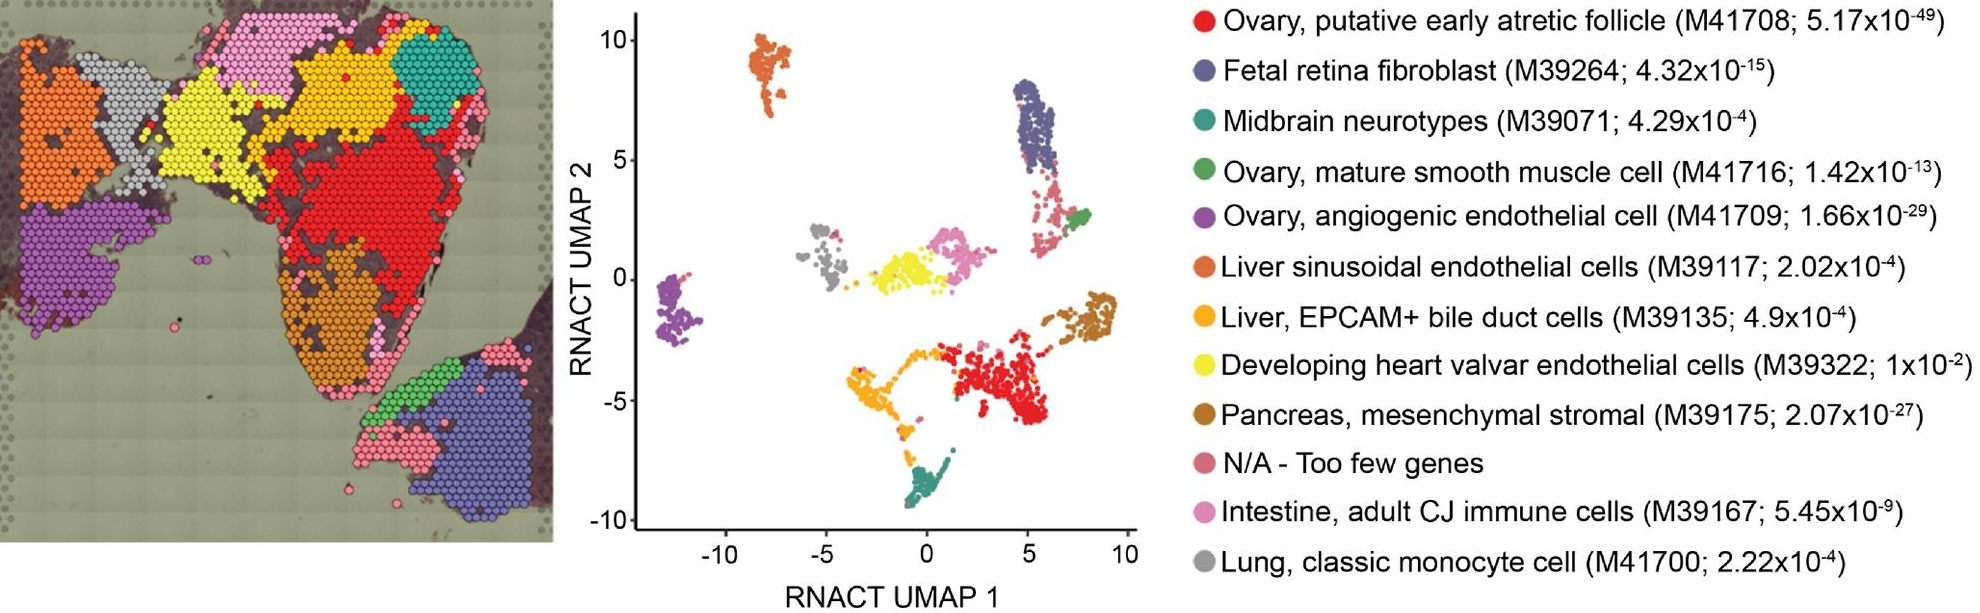
\includegraphics[width=\textwidth]{images/Sanders_Fig3B.png}
    \caption{\citet{sanders_small_2022} clustering of cell types mapped to tumor section and UMAP plot of cell type clusters, with highest enriched cell marker annotation per cluster.}
    \label{fig:Sanders_tissuefig}
\end{figure}

The GEO deposited data included raw SpaceRanger outputs such as counts and spatial transcriptomics imaging files, as well as a metadata table containing a portion of the downstream analysis. Details for the original \citet{sanders_small_2022} analysis are provided in ``Methods". Notably, the final SCTransform clustering and gene set enrichment results as presented in the publication were not included in the metadata in the GEO accessible data. A metadata column described 15 unique `SCT clusters', but it was inferred that clusters in the final publication were a result of alternate clustering methodologies that were difficult to replicate given that the reference publication metadata that \citet{sanders_small_2022} used when constructing and annotating clusters was not available.

To reconcile the downloaded data with the publication data, we reanalyzed the downloaded data as closely as possible to the \citet{sanders_small_2022} GitHub repository. The result of rerunning the standard Seurat SCTransform spatial transcriptomics analysis pipeline (referred to as `SCTrr') can be seen in Supplementary Fig. \ref{fig:SCTcl_rr}, where the rerun cluster boundaries largely match the SCTransform clusters as reported in the GEO metadata.

\subsubsection*{Spatially aware dimensional reduction comparison}

We then integrated spatially aware dimensional reduction into the Seurat spatial transcriptomics pipeline and compared the resulting differences in the PCA results, a common first step in downstream spatial transcriptomics analysis. As described in the ``Methods" section, two variants of spatial PCA was run, one with variable gene selection via SPARK\citep{sun_statistical_2020} and the other with using the result of Seurat `FindVariableFeatures' (`SVF', ``Seurat Variable Features").

As seen in Fig. \ref{fig:DimPlotPCA}, notable differences already arise upon the application of spatially aware PCA. There is a notable difference between the standard PCA of SCTrr compared to the SpatialPCA results, with clusters appearing less separate from each other. The application of SpatialPCA suggests that by incorporating spatial information as a factor during PCA, the cells within the sample may not be separable given their location on the physical tissue slide and may be comprised of similar gene expression profiles. Location-agnostic methods such as standard PCA ignores the positional context for each cell spot, so it intuitively follows that the clusters may be more separable at the cost of potentially not replicating real life tissue morphology.

\begin{figure}[h!]
    \centering
    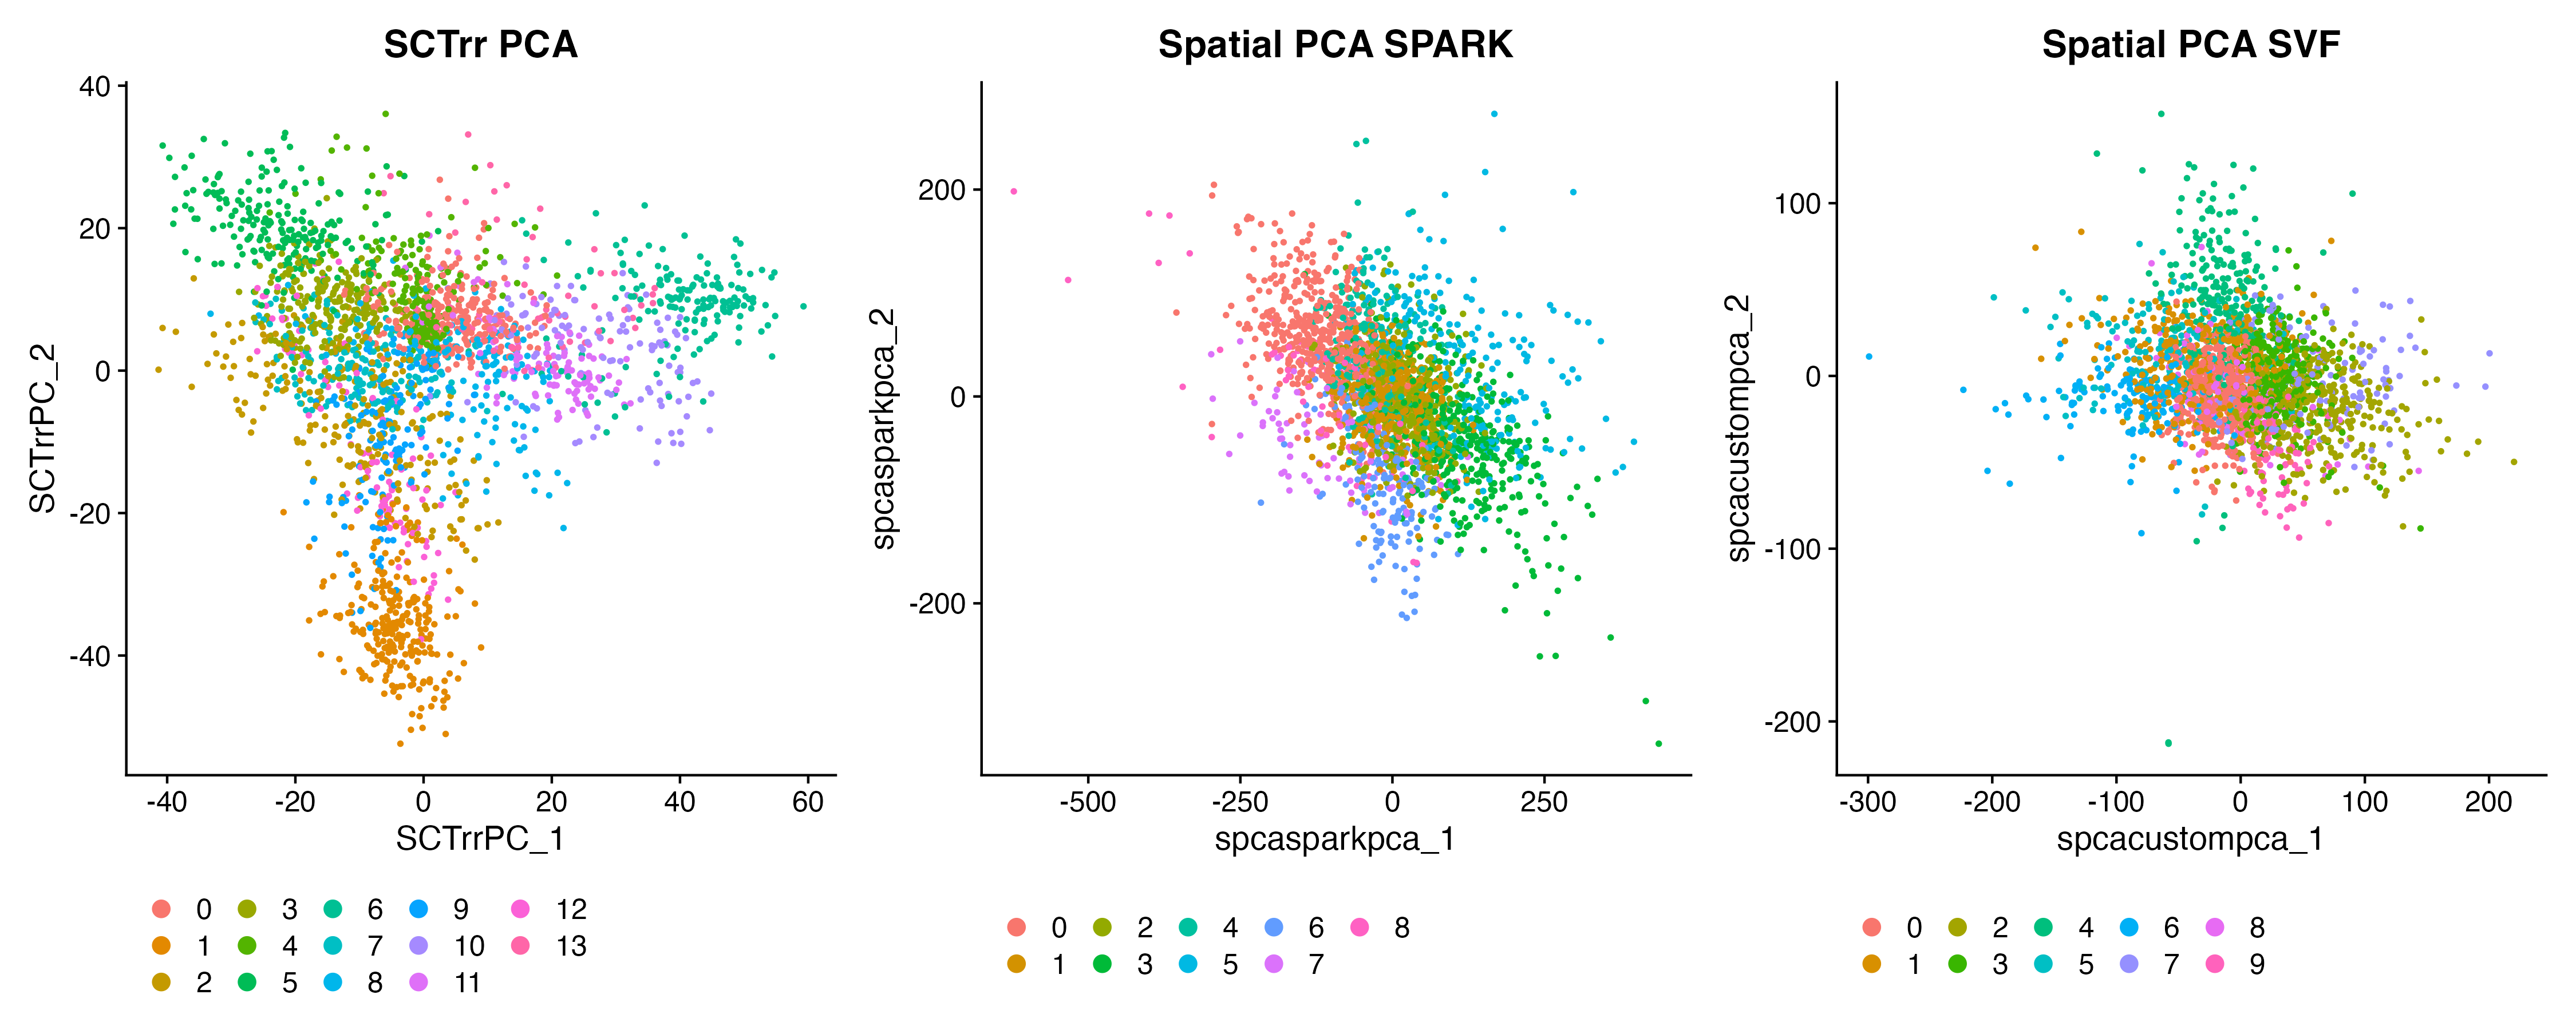
\includegraphics[width=\textwidth]{images/DimPlotPCA_D_GTFB1170_SmallCellOvarianCancer_pw_strip.png}
    \caption{PCA dimensional reduction plots comparing the result of PCA applied to SCTransformed data (SCTrr) (left) with SpatialPCA applied with either SPARK (center) or Seurat Variable Features (SVF) (right) variable genes, colored by cluster number.}
    \label{fig:DimPlotPCA}
\end{figure}

Uniform manifold approximation and projection (UMAP)\citep{mcinnes_umap_2020}, a non-linear dimensional reduction visualization technique, is commonly incorporated in spatial transcriptomics analysis. UMAP is performed upon PCA results, so we applied UMAP to the previous four PCA results and visualized the plot with grouping by cluster. As seen in Fig. \ref{fig:DimPlotUMAP}, the ``SCTrr UMAP" shapes appear to resemble the shapes in the UMAP results published in \citet{sanders_small_2022} (Fig. \ref{fig:Sanders_tissuefig}), validating our replication of the published data. Similar to the differences between standard PCA and SpatialPCA in Fig. \ref{fig:DimPlotPCA}, the clusters in the SpatialPCA UMAP results appear less separated and are often overlapping, even if the clusters are easier to identify by eye in the UMAP plots compared to the PCA plots.

\begin{figure}[h!]
    \centering
    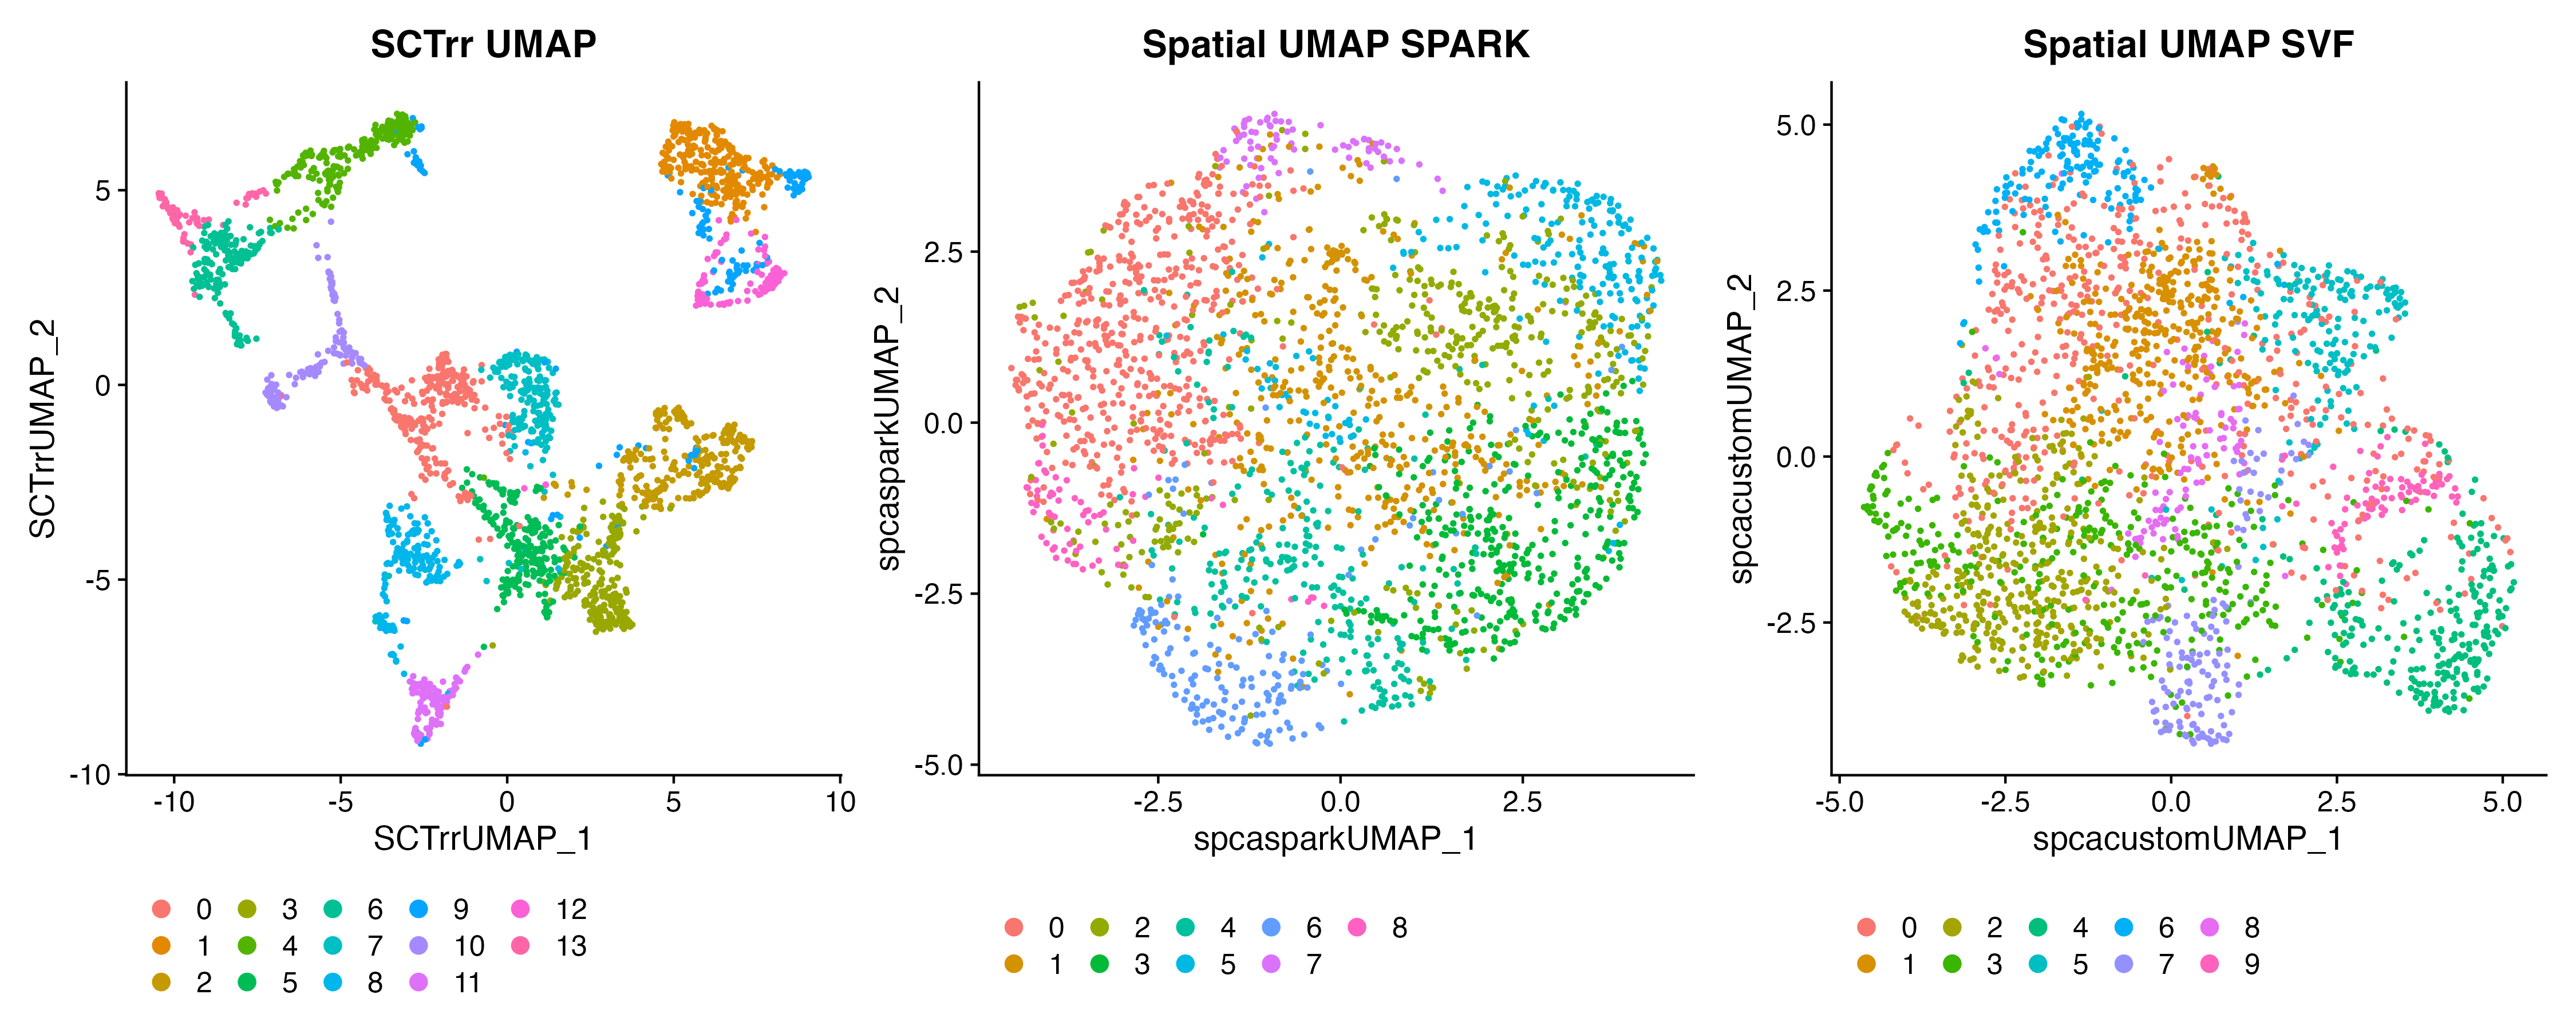
\includegraphics[width=\textwidth]{images/DimPlotUMAP_D_GTFB1170_SmallCellOvarianCancer_pw_strip.png}
    \caption{UMAP dimensional reduction plots comparing the result of UMAP ran with standard PCA applied to SCTransformed data (SCTrr) (left) with UMAP ran with SpatialPCA applied with either SPARK (center) or SVF (right) variable genes , colored by cluster annotation.}
    \label{fig:DimPlotUMAP}
\end{figure}

Further replicating \citet{sanders_small_2022} analysis, we visualized the SpatialPCA captures spot clustering results overlaid on the tissue slide. In the Seurat analysis workflow, clusters of cells are identified by applying the Louvain clustering algorithm on a shared nearest neighbor (SNN) graph modularity optimization built upon PCA dimensionality reduction. For data processed through SpatialPCA, we built the SNN graph based on spatial principal components to detect clusters at a resolution of 0.8. As seen in Fig. \ref{fig:SpatialPlotCl}, there is a striking difference between the clustering patterns from SpatialPCA dimensional reduction compared to the clustering based on standard PCA (Supp. Fig. \ref{fig:SCTcl_rr}, Fig. \ref{fig:Sanders_tissuefig}). Even with a higher resolution setting of 0.8 compared to the original setting of 0.6, only 8 and 10 clusters were found through SpatialPCA compared to 12 SCTrr clusters. The SpatialPCA results appear spotted or striped, with alternating cluster annotations in certain regions of the tissue slice. Even with the spotted cluster patterning, clusters are focally concentrated, such as in the SPARK results (Fig. \ref{fig:SpatialPlotCl}, left), where cluster 8 (hot-pink) is only present in the tissue region near the center of the slice, and cluster 6 (royal blue) is mainly present in the bottom right of the tissue slice. The SVF SpatialPCA clusters (Fig. \ref{fig:SpatialPlotCl}, right) correspond better than SPARK clusters to the SCTrr clusters, with the SpatialPCA SVF cluster 7 (purple) and cluster 5 (turquoise) comprising a section of the tissue near the middle of the slide that corresponds to SCTrr cluster 2.

\begin{figure}[h!]
    \centering
    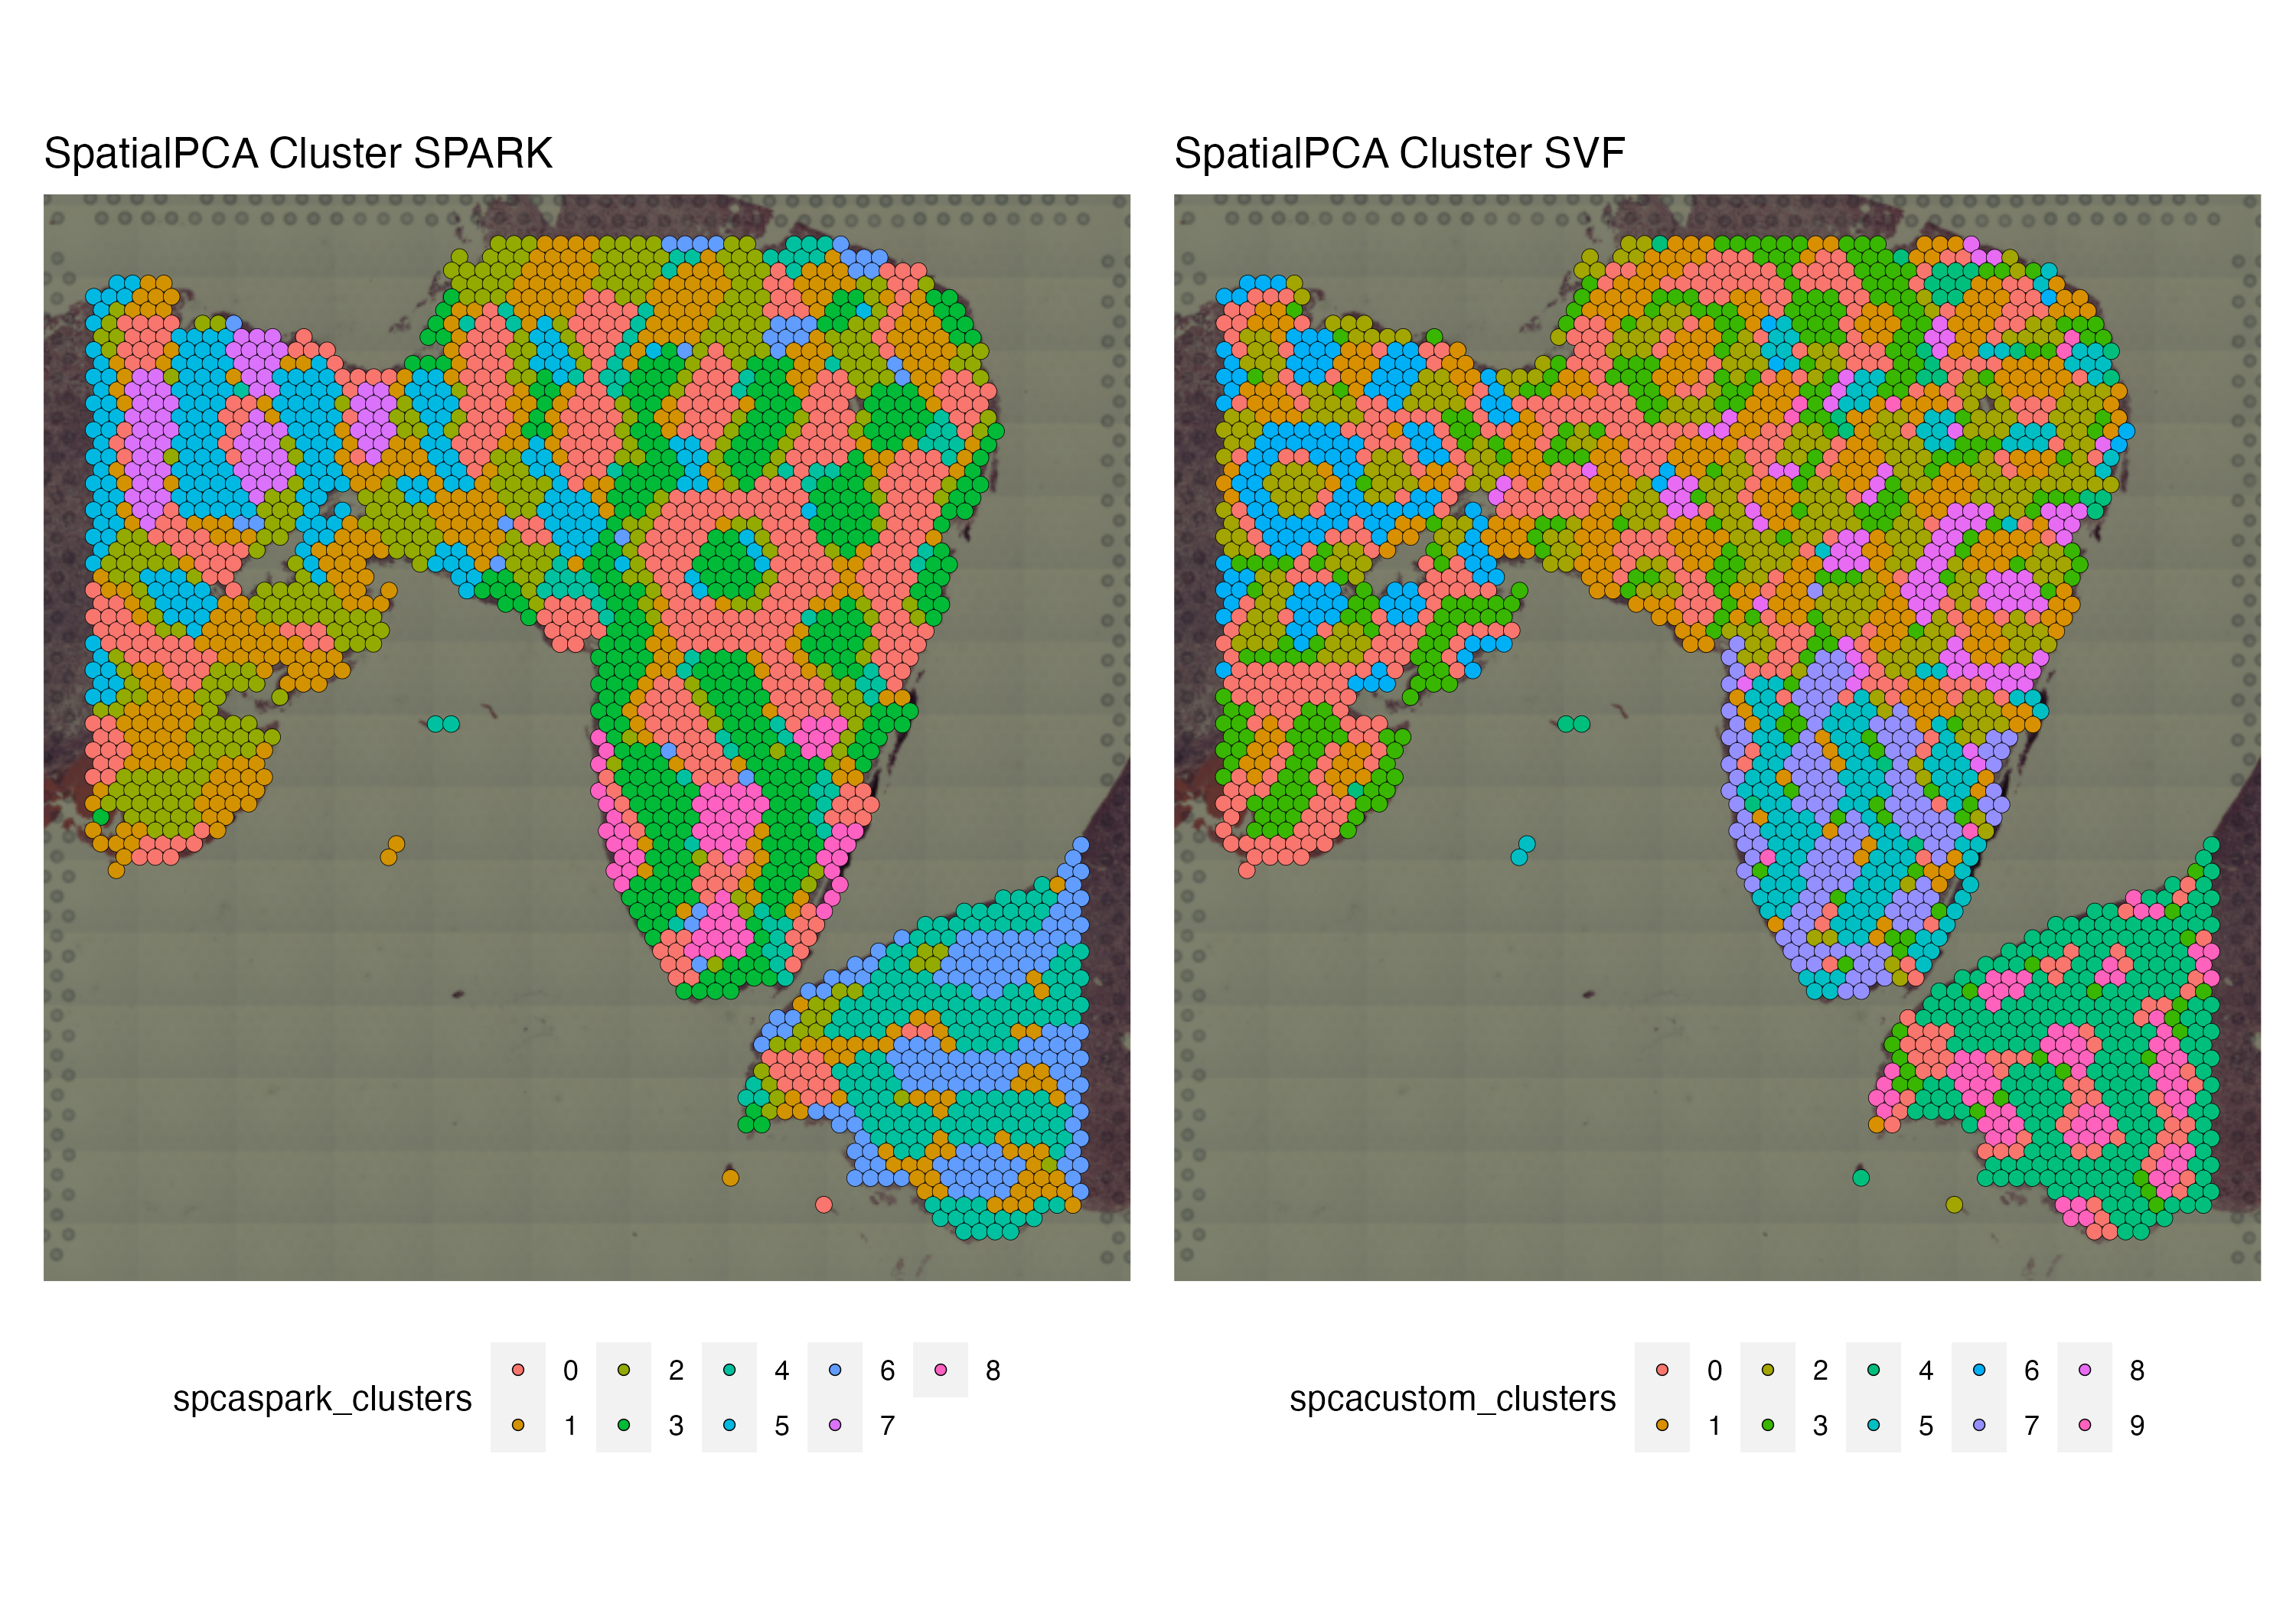
\includegraphics[width=\textwidth]{images/SpatialDimPlot_D_GTFB1170_SmallCellOvarianCancer_pw_clusters_spcasparksvf.png}
    \caption{SpatialPCA capture spot clustering results overlaid on tissue slide image.}
    \label{fig:SpatialPlotCl}
\end{figure}

\subsubsection*{Spatial PCA cluster cell type annotation}

As seen in \ref{fig:Sanders_tissuefig}, clusters in the original publication were annotated with cell type signatures by using the `clustifyr'\citep{fu_clustifyr_2020}, which assigns cell types to single-cell RNA sequencing by using a correlation-based approach and leveraging an external reference. The \citet{sanders_small_2022} paper used \citet{olalekan_characterizing_2021}, a paper analyzing the tumour micro-environment of metastatic ovarian cancer by Drop-seq single-cell transcriptomics, as reference to annotate the tumour sample. However, the cell-type annotation metadata for \citet{olalekan_characterizing_2021} was missing in the data deposits for either publication.

We used SingleR\citep{aran_referencebased_2019}, a correlation-based R package (see `Methods'), to perform cell-type annotation of individual capture spots (Fig. \ref{fig:SRSpot}, top left) based on the Human Primary Cell Atlas\citep{mabbott_expression_2013} reference. Ten different cell types were detected with individual cell types not cleanly separating into spatial domains. The clustering results for SCTrr and SpatialPCA also generally do not cleanly separate the annotated cell-spot types into individual clusters with the exception of SCTrr cluster 6, SPARK cluster 6 and 7, and SVF cluster 6 that are comprised of a higher proportion of neuron-like cells. Those neuron-high clusters can be seen to be spatially located in the same area near the top-left of the tissue slide (Supp. Fig. \ref{fig:SCTcl_rr}, Fig. \ref{fig:SpatialPlotCl}). 

\begin{figure}[h!]
    \centering
    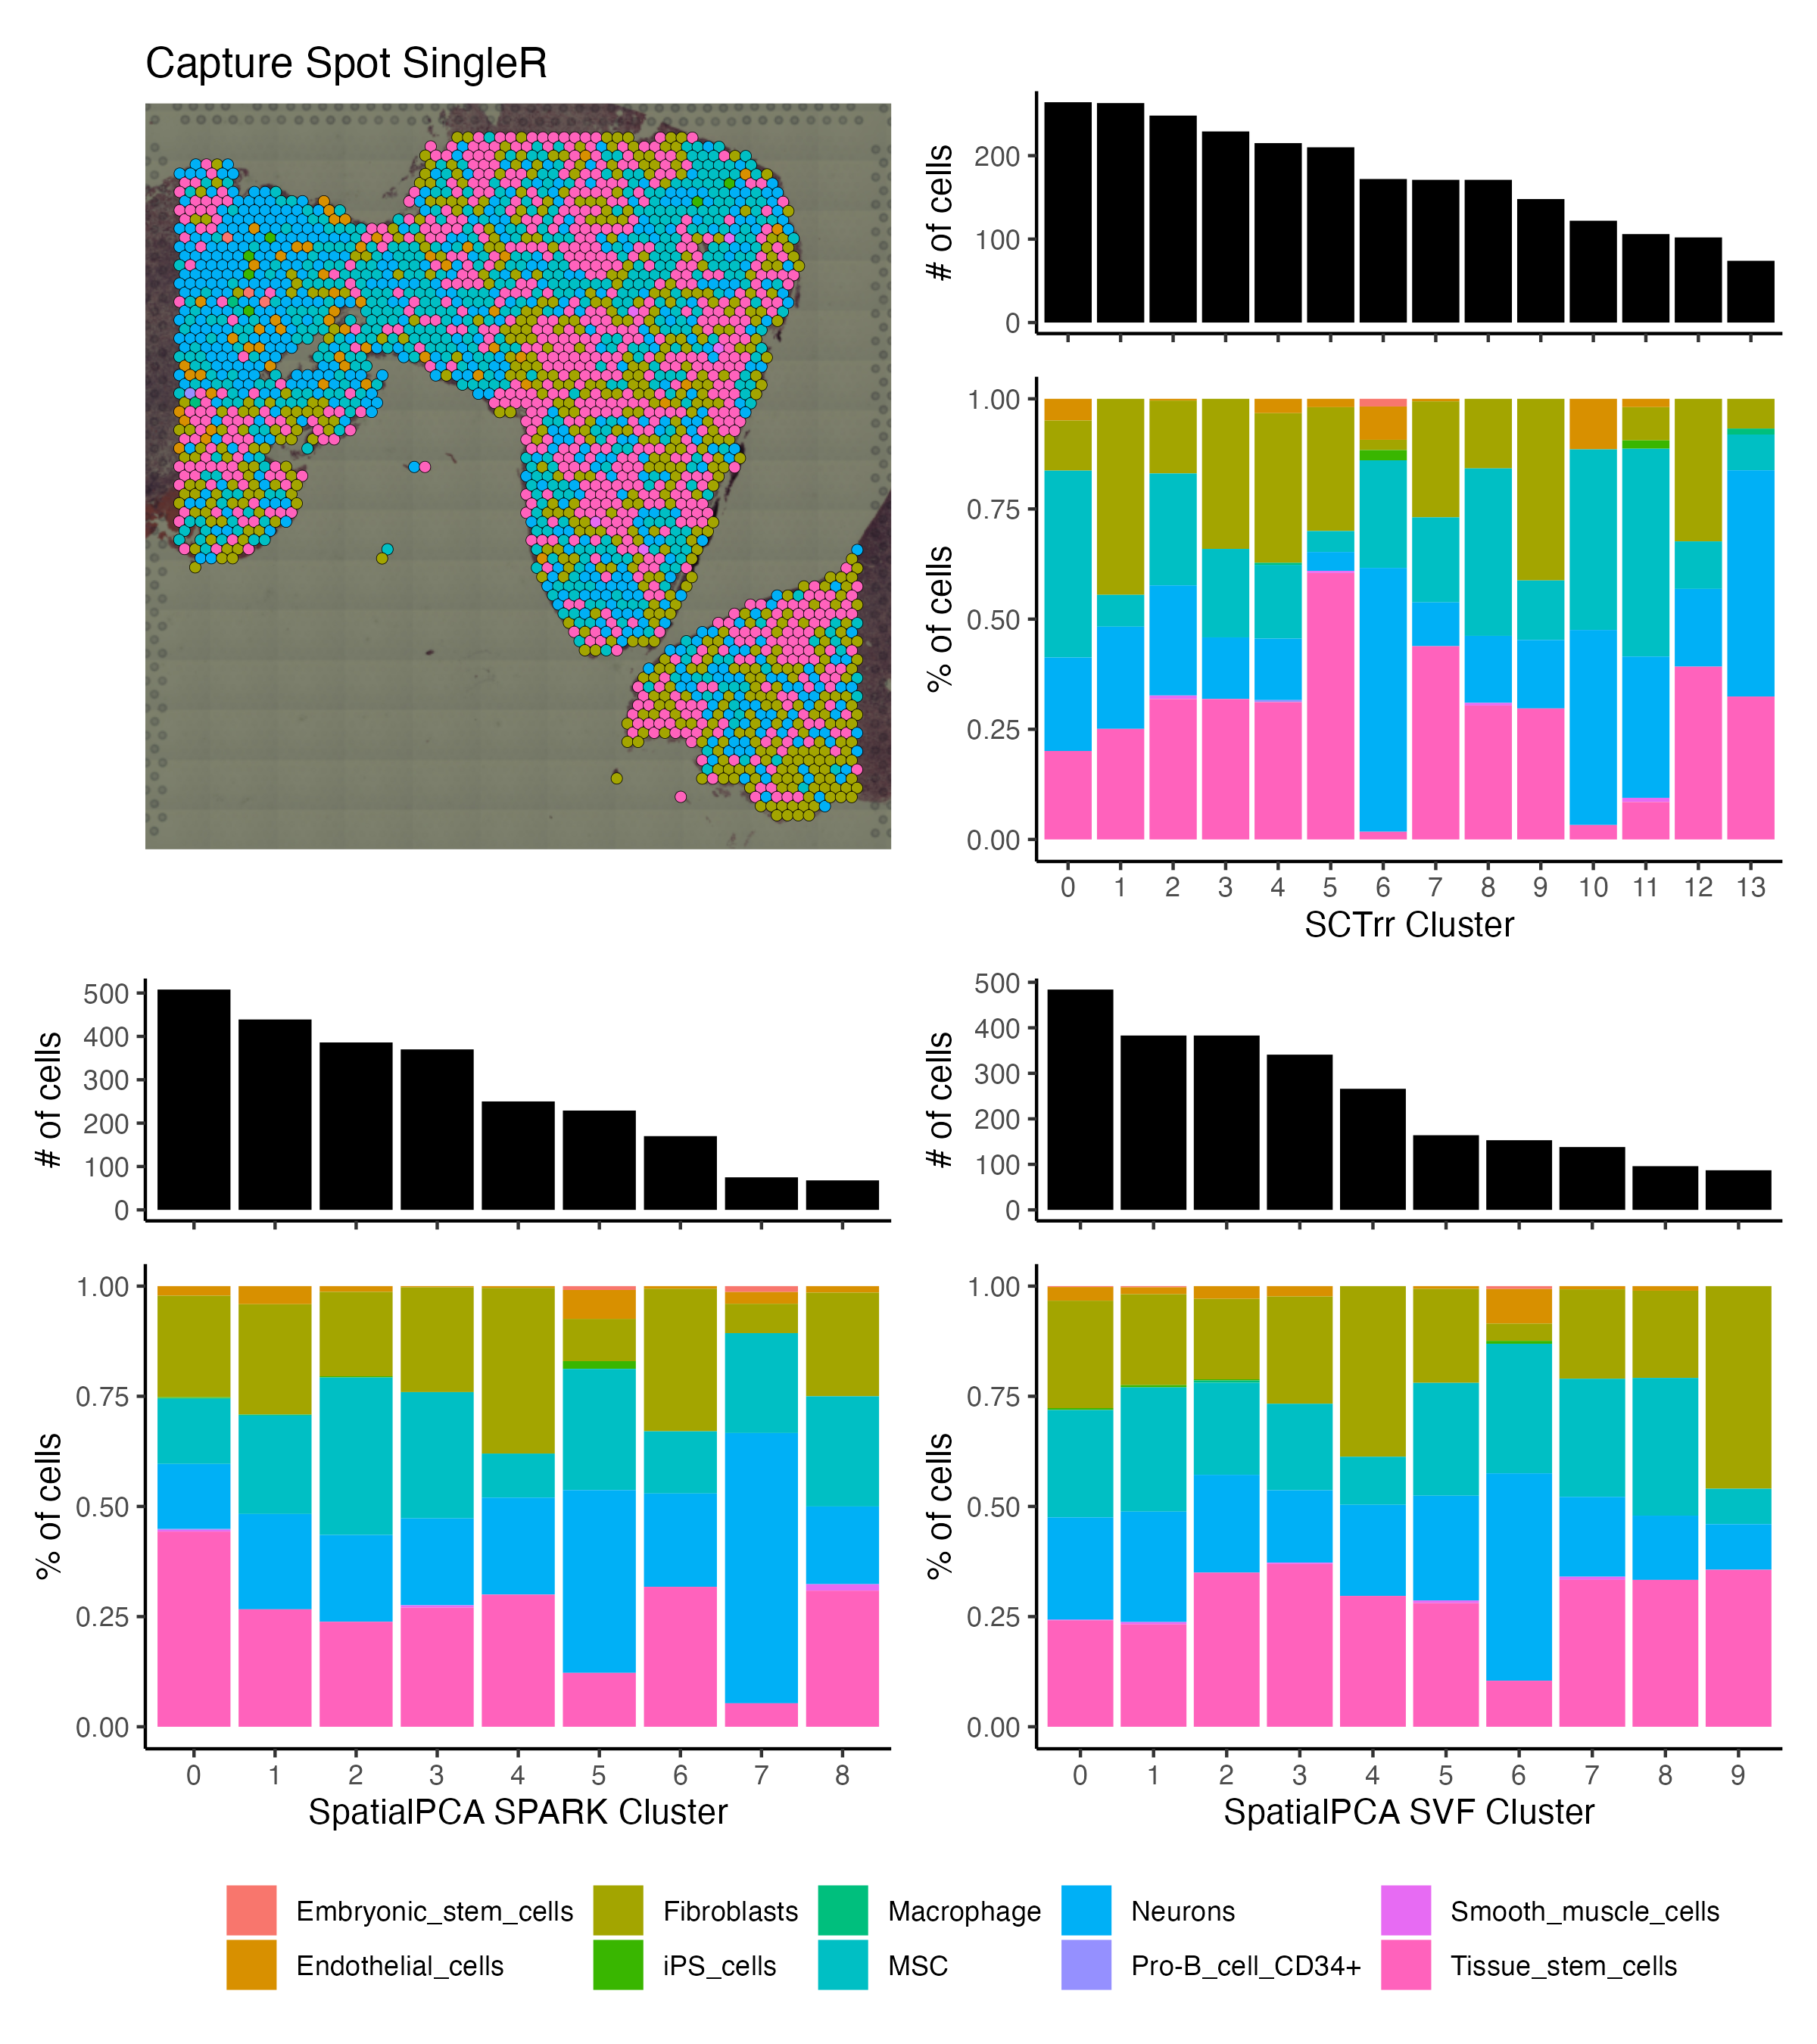
\includegraphics[width=\textwidth]{images/SRSpot_D_GTFB1170_SmallCellOvarianCancer_pw_sq.png}
    \caption{Capture spot specific SingleR annotation. Cell-type specific annotation spatial plot on top-left, and cluster cell-type composition bar plots for the rest of the plots.}
    \label{fig:SRSpot}
\end{figure}

We reproduced a similar effect to \citet{sanders_small_2022} of cluster type annotation by using the correlation-based SingleR to annotate aggregate gene expression profiles per cluster (Fig. \ref{fig:SRCluster}). The 14 unique SCTrr clusters were assigned to only 4 unique cell types: fibroblasts, mesenchymal stem cells (MSCs), neurons, and tissue stem cells. The SpatialPCA-based clusters were assigned more diverse cell types, including chondrocytes, erythroblasts, monocytes, and B-cells. 

Comparing these cluster annotations to the \citet{sanders_small_2022} annotations, certain regions appear to correspond well, such as the publication (Fig. \ref{fig:Sanders_tissuefig}) attributing a section of the bottom right slide to "Ovary, mature smooth muscle cell", and the SpatialPCA SPARK results denote clusters in that same region as fibroblasts. A recent publication\citep{zhang_role_2022} has noted the importance of fibroblasts in the ovarian cancer tumour micro-environment and its relation with smooth muscle cells that able to trans-differentiate into cancer-associated fibroblasts. Interestingly, out of all cluster annotations, only the Spatial PCA results from using spatially expressed genes as detected by SPARK hint at this relationship between fibroblasts and the smooth muscle cells as annotated in the Sanders paper.

Another biological finding highlighted in the \citet{sanders_small_2022} paper was the prevalence of clusters predicted to be involved in angiogenesis and endothelial cell biology. Increased endothelial cell proliferation have been linked to angiogenic signals in literature\citep{munoz-chapuli_angiogenesis_2004}. The Spatial PCA results relate to this finding, with large regions overlapping the Sanders endothelial cell regions annotated as chondrocytes, which have been linked to vascular endothelial growth factors that promote the migration of vascular endothelial cells\citep{xiaoshi_setd7_2021}, and erythroblasts, which have also been shown to be a source of angiogenic factors. The lower resolution of cell type annotation for SCTrr clusters result in an inability to predict the presence more specific cell types that may provide additional biological insights.

\begin{figure}[h!]
    \centering
    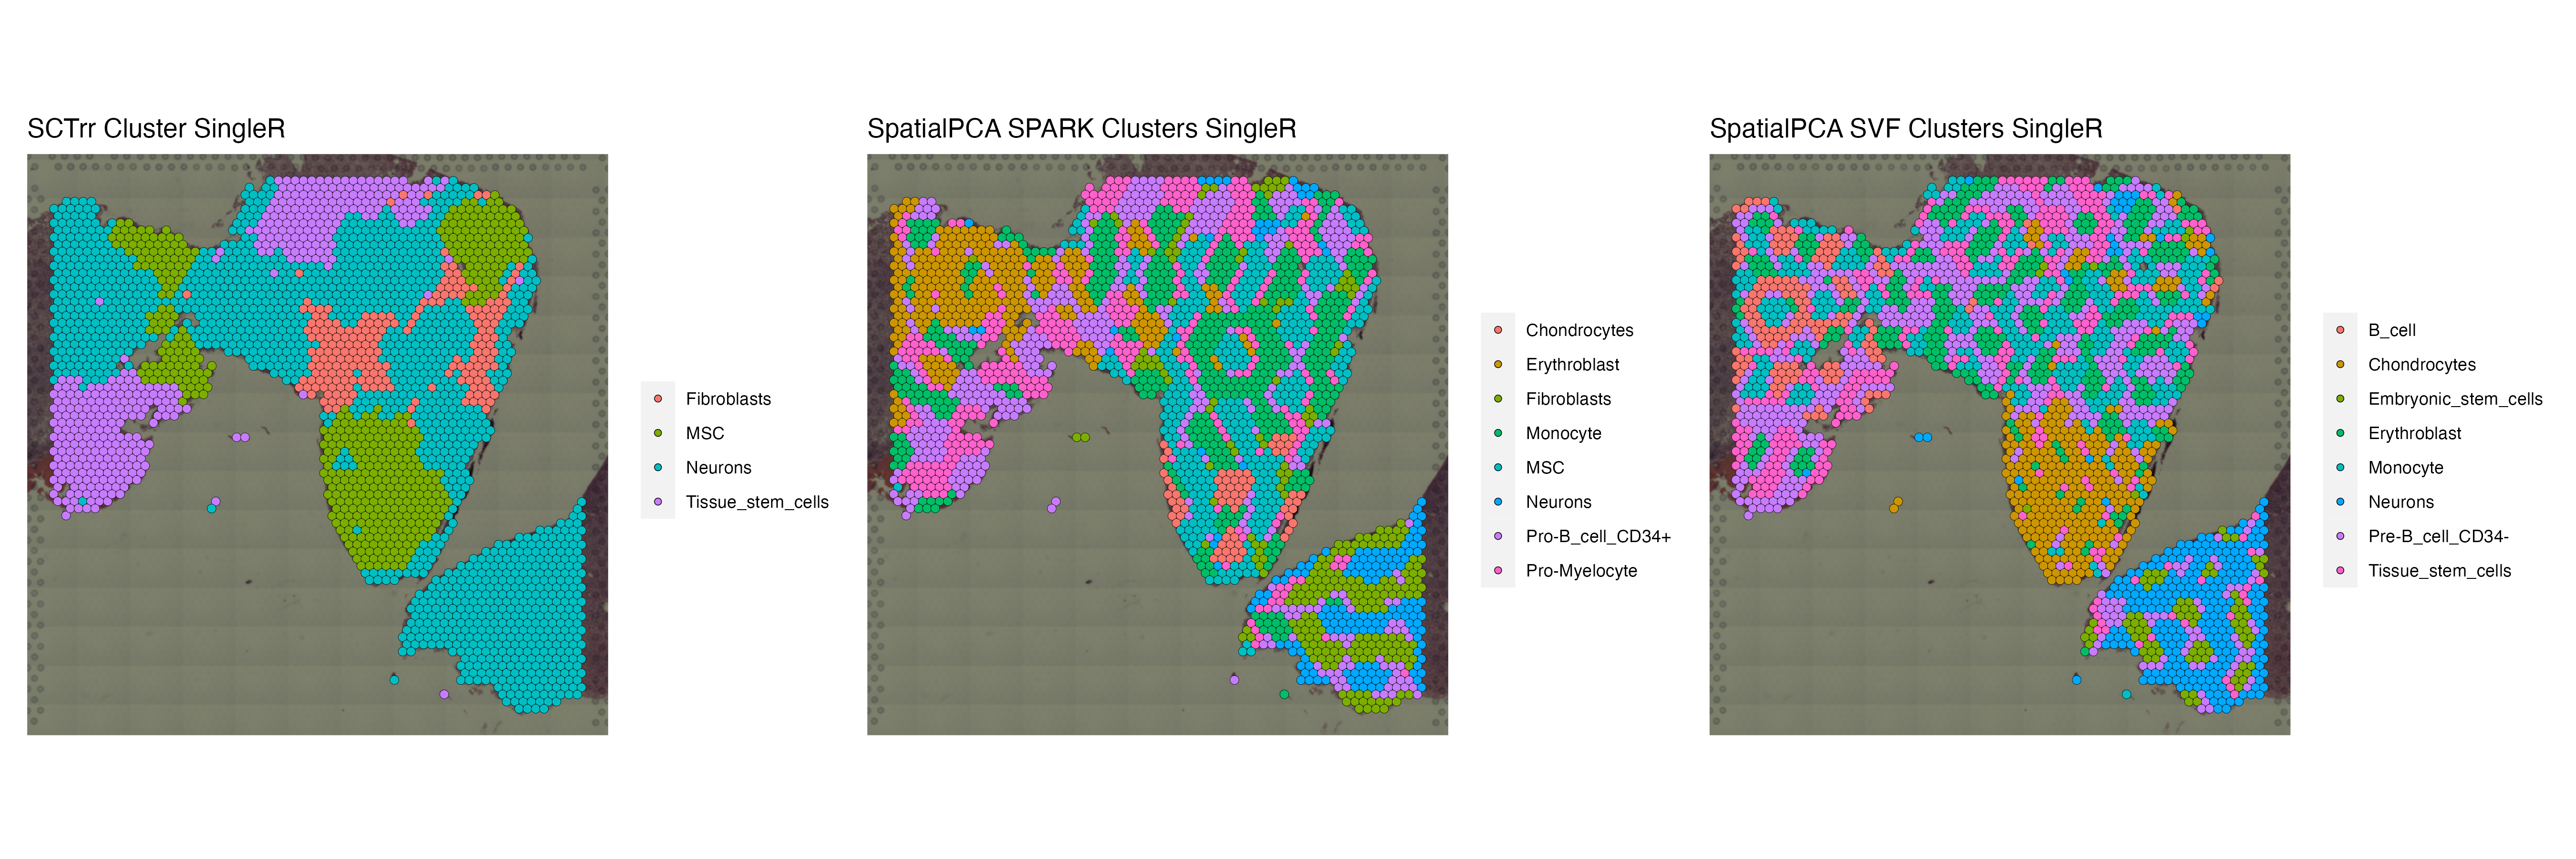
\includegraphics[width=\textwidth]{images/SRCluster_D_GTFB1170_SmallCellOvarianCancer_pw_sq.png}
    \caption{Cluster specific SingleR annotation.}
    \label{fig:SRCluster}
\end{figure}

\section*{Discussion}

We have explored the impact of spatially aware dimensional reduction by applying SpatialPCA to both simulated data as well as real patient cancer data.

The results from simulation indicate that SpatialPCA does an acceptable job, however, the similarity between domains B and D were tough for the algorithms to distinguish. This is likely a consequence of using just 10 high-signal marker genes and intentionally making domains B and D similar. We are left wondering however: did this simulation make domains that were too similar? i.e. Was this still representative of biology? The differences in similar celltypes is subtle in real biology, and so modelling these minutiae with negative binomial models (or the other options we looked at ZINB, poisson etc.) is a hard problem. 

There is a clear opportunity for future work here: modelling similar domains from real reference data. The story told by the CHAOS score values tell a similar story: that our test data-set should probably be a bit more complex. With SRTsim we can use scRNAseq data (of which there is considerably more freely available online) to fit models and use as priors in the SIMsrt workflow of simulating specific domains. Combining these bespoke domains together with other simulated domains to create the full simulated data-set would then likely represent a better test-set to understand and document the capabilities of methods such as SpatialPCA. 

Finally, for the simulated data portion of our study, we would like to note that a significant limiting factor was the use-ability of the the SRTsim UI. This software had clearly not been tested too much and bugs were common. The R-functions being called in the background were more powerful, and allowed for more granular attention in simulations, but the documentation for these functions was somewhat lacking. These two issues lead to time-constraints that would likely be overcome in future work.

Applying spatially aware dimensional reduction to the ovarian cancer dataset resulted in markedly different dimensional reduction results, which further impacted downstream clustering patterns. The \citet{sanders_small_2022} study presented an interesting opportunity for application of a more cutting edge analysis, given its qualities of being a relatively recent paper focused on a more clinical perspective rather than bioinformatics innovation. Similar to other translationally focused papers, many aspects of its analysis code such as the core PCA, clustering, and UMAP steps appear to be adapted directly from Seurat vignettes.

The application of spatially aware dimensional reduction, however, did not provide clear indications of analytical benefits relative to the conclusions drawn from the original paper. One of \citet{sanders_small_2022}'s main conclusions is shown in Figure \ref{fig:Sanders_tissuefig}, where the cell type annotations appear to have been manually curated from gene set enrichment results. Without access to the complete detailed methods needed to replicate the manual cluster annotations, we instead relied on unsupervised cell type annotation using an similarly correlation-based cell type annotation method. Unsupervised analysis affords certain advantages such as increased reproducibility and less selection bias, but ultimately a literature-based interpretation of results is still required to derive biological conclusions.

The less clearly distinct clustering patterns from the Spatial PCA results also raises questions as to whether ``cleaner" clustering results from the standard PCA pipeline may be over-simplifying real cell-type heterogeneity in tissue sections. Biologically, real ovarian cancers samples may not have as clearly distinctive cell-type spatial domains as other tissue types. The lack of a ground truth in real samples means that using a positive control such as glandular structures that may afford stronger conclusions. However, it was exceedingly difficult to find a dataset in the current publication landscape that fit our criteria of having the minimum data required to appropriately load in for Seurat analysis. Many real datasets we attempted to analyze were missing parts of SpaceRanger analysis, or missing cell metadata tables, and only uploaded a raw counts matrix without spatial information even if the publication focused on spatial transcriptomics analysis. This highlights a large, still growing issue, regarding lack of reproducibility in public datasets that is only starting to be addressed in the field\citep{fullgrabe_guidelines_2020}.

\section*{Methods}

\subsection*{Simulation benchmarking}

The cells for this tissue were generated/simulated according to the GitHub guide for SRTsim \citep{SRTsim_vig}. 1359 cells were simulated with fold changes of just 2 or 3 separating each tissue. For each domain 10 higher-signal marker genes, 50 lower-signal marker genes, and 7000 noise genes were simulated using a negative binomial model. 

We then ran SpatialPCA using the default workflow/params as described in their paper on the gland-test dataset and subsequently performed walktrap clustering on the top 20 spatial components. Walktrap was run using 3, 4 and 5 expected clusters. We evaluated the performance of SpatialPCA using LISI, Silhouette, and CHAOS scores.

CHAOS and LISI scores we calculated using the functions published in the Spatial PCA package. The average silhouette width for each domain was found by first calculating the minkowski distance courtesy of the `dist` function from the 'stats' R-package between the top 20 spatial PCs and then using the silhouette function from 'cluster' R-package. 

\subsection*{Ovarian cancer spatial transcriptomics data}

We integrated the SpatialPCA workflow to a publicly available set of 8 human ovarian cancer tissue samples (GEO Series GSE213699) that were analyzed using the Visium 10x spatial RNA-seq platform. The samples were collected from different anatomical sites and therapy statuses, such as small cell ovarian, ovarian, and omentum tumours.

As described in \citet{sanders_small_2022}, formalin-fixed paraffin-embedded (FFPE) tumour tissues were prepared using the Visium Spatial Expression protocols, with resulting sequencing data was processed through the 10x Genomics SpaceRanger software to assign tissue location and gene expression values.

The SpaceRanger raw data was then read into Seurat \citep{hao2021} and data normalized with the `SCTransform' function with default values. `SCTransform'\citep{choudhary_comparison_2022}, as recommended by Seurat for spatial transcriptomics analysis, is a modelling framework that can normalize and variance stabilize molecular count data in scRNA-seq experiments to improve downstream analytical tasks. Dimensionality reduction was performed on spots with `RunPCA' and`RunUMAP', with number of principal components used for UMAP determined by visualizing an elbow plot. Clusters were identified using Seurat `FindNeighbors' and `FindClusters' with a resolution of 0.6.

Function `make\_sobj' was created to correctly access the raw data downloaded from GEO and wrangle the data to a format loadable by Seurat `Load10X\_Spatial' per ovarian cancer sample.

\subsubsection*{Incorporating spatially aware dimensional reduction to ovarian cancer analysis}

For sample `D-GTFB1170', clustering results similar to \citet{sanders_small_2022} were produced by closely following the analysis code from the paper (https://github.com/kwells4/visium\_ovarian\_cancer). Using the Seurat package, the same functions and parameters for certain steps of the workflow, such as number of principal components used for dimensional reduction and clustering resolution, were chosen. Function `process\_sobj' was created to run the standard `SCTransform` based spatial transcriptomics processing Seurat pipeline per ovarian cancer sample.

SpatialPCA, using \citet{shang2022}'s R package, was applied to sample `D-GTFB1170' following their DLPFC Visium analysis tutorial (https://lulushang.org/SpatialPCA\_Tutorial/DLPFC.html) in the function `process\_SPCA'. Two SpatialPCA objects were created, one with using spatially expressed variable genes detected by the SPARK method\citep{sun_statistical_2020}, default for smaller datasets, and another using Seurat's `VariableFeatures` (SVF) genes as a custom gene list. SPARK employs generalized linear spatial models to directly model non-Gaussian spatial count data, while Seurat `FindVariableFeatures' selects top variable by fitting a local polynomial regression line to the relationship of log(variance) and log(mean).

A kernel matrix using spatial locations (`SpatialPCA\_buildKernel') was then built for each SpatialPCA object, with `kerneltype' set as Gaussian and `bandwidthtype' set to the \citet{sheather_reliable_1991a} method as recommended for smaller sized datasets. Using `SpatialPCA\_EstimateLoading', loading matrices were calculated according to default parameters and spatial principal components (latent factor matrix Z) were then derived. Both variants of the SpatialPCA dimensional reduction results were then incorporated to the Seurat object, and clustering performed at a resolution of 0.8 and the first 20 spatial PCs used to calculate UMAP dimensional reduction.

\subsubsection*{SingleR cell and cluster type annotation}

The SingleR\citep{aran_referencebased_2019} R package was used to perform unbiased cell type annotation of individual capture spots and capture spot clusters. The algorithm uses built-in references from the Human Primary Cell Atlas\citep{mabbott_expression_2013} to identify marker genes from the reference and compute assignment scores based on the Spearman correlation across markers for each input cell against the label in the reference. The highest assignment score is the cell-type assigned to the cell. Cluster-level annotation was performed by inputting the cluster annotations to SingleR so transcriptomics profile per cluster were aggregated and annotation performed on cluster-level profiles. Default parameters were used.

\subsubsection*{Visualization}
Clustering, PCA, and UMAP results were visualized using `ggplot2'\citep{wickham_ggplot2_2009}, `patchwork'\citep{pedersenthomasl_patchwork_2023}, and `Seurat'\citep{hao2021} R packages.

\subsection*{Code and Data Availability}

Code underlying the simulation and ovarian cancer spatial analysis is uploaded to a GitHub repository at: https://github.com/liaoyjruby/CPSC545\_Project

The input data and output results for this project is accessible via a UBC organization account in a OneDrive folder: 

https://ubcca-my.sharepoint.com/:f:/g/personal/liaoyj\_student\_ubc\_ca/ \\ Eligh\_HNUKJMivdN98tB1QUBsA8HAcL7yn6IXLkP2gkHkA?e=DHj8aT

\newpage

\bibliography{CPSC545_ProjectRefs}

\newpage

\section*{Supplementary Figures}

\begin{figure}[h!]
    \centering
    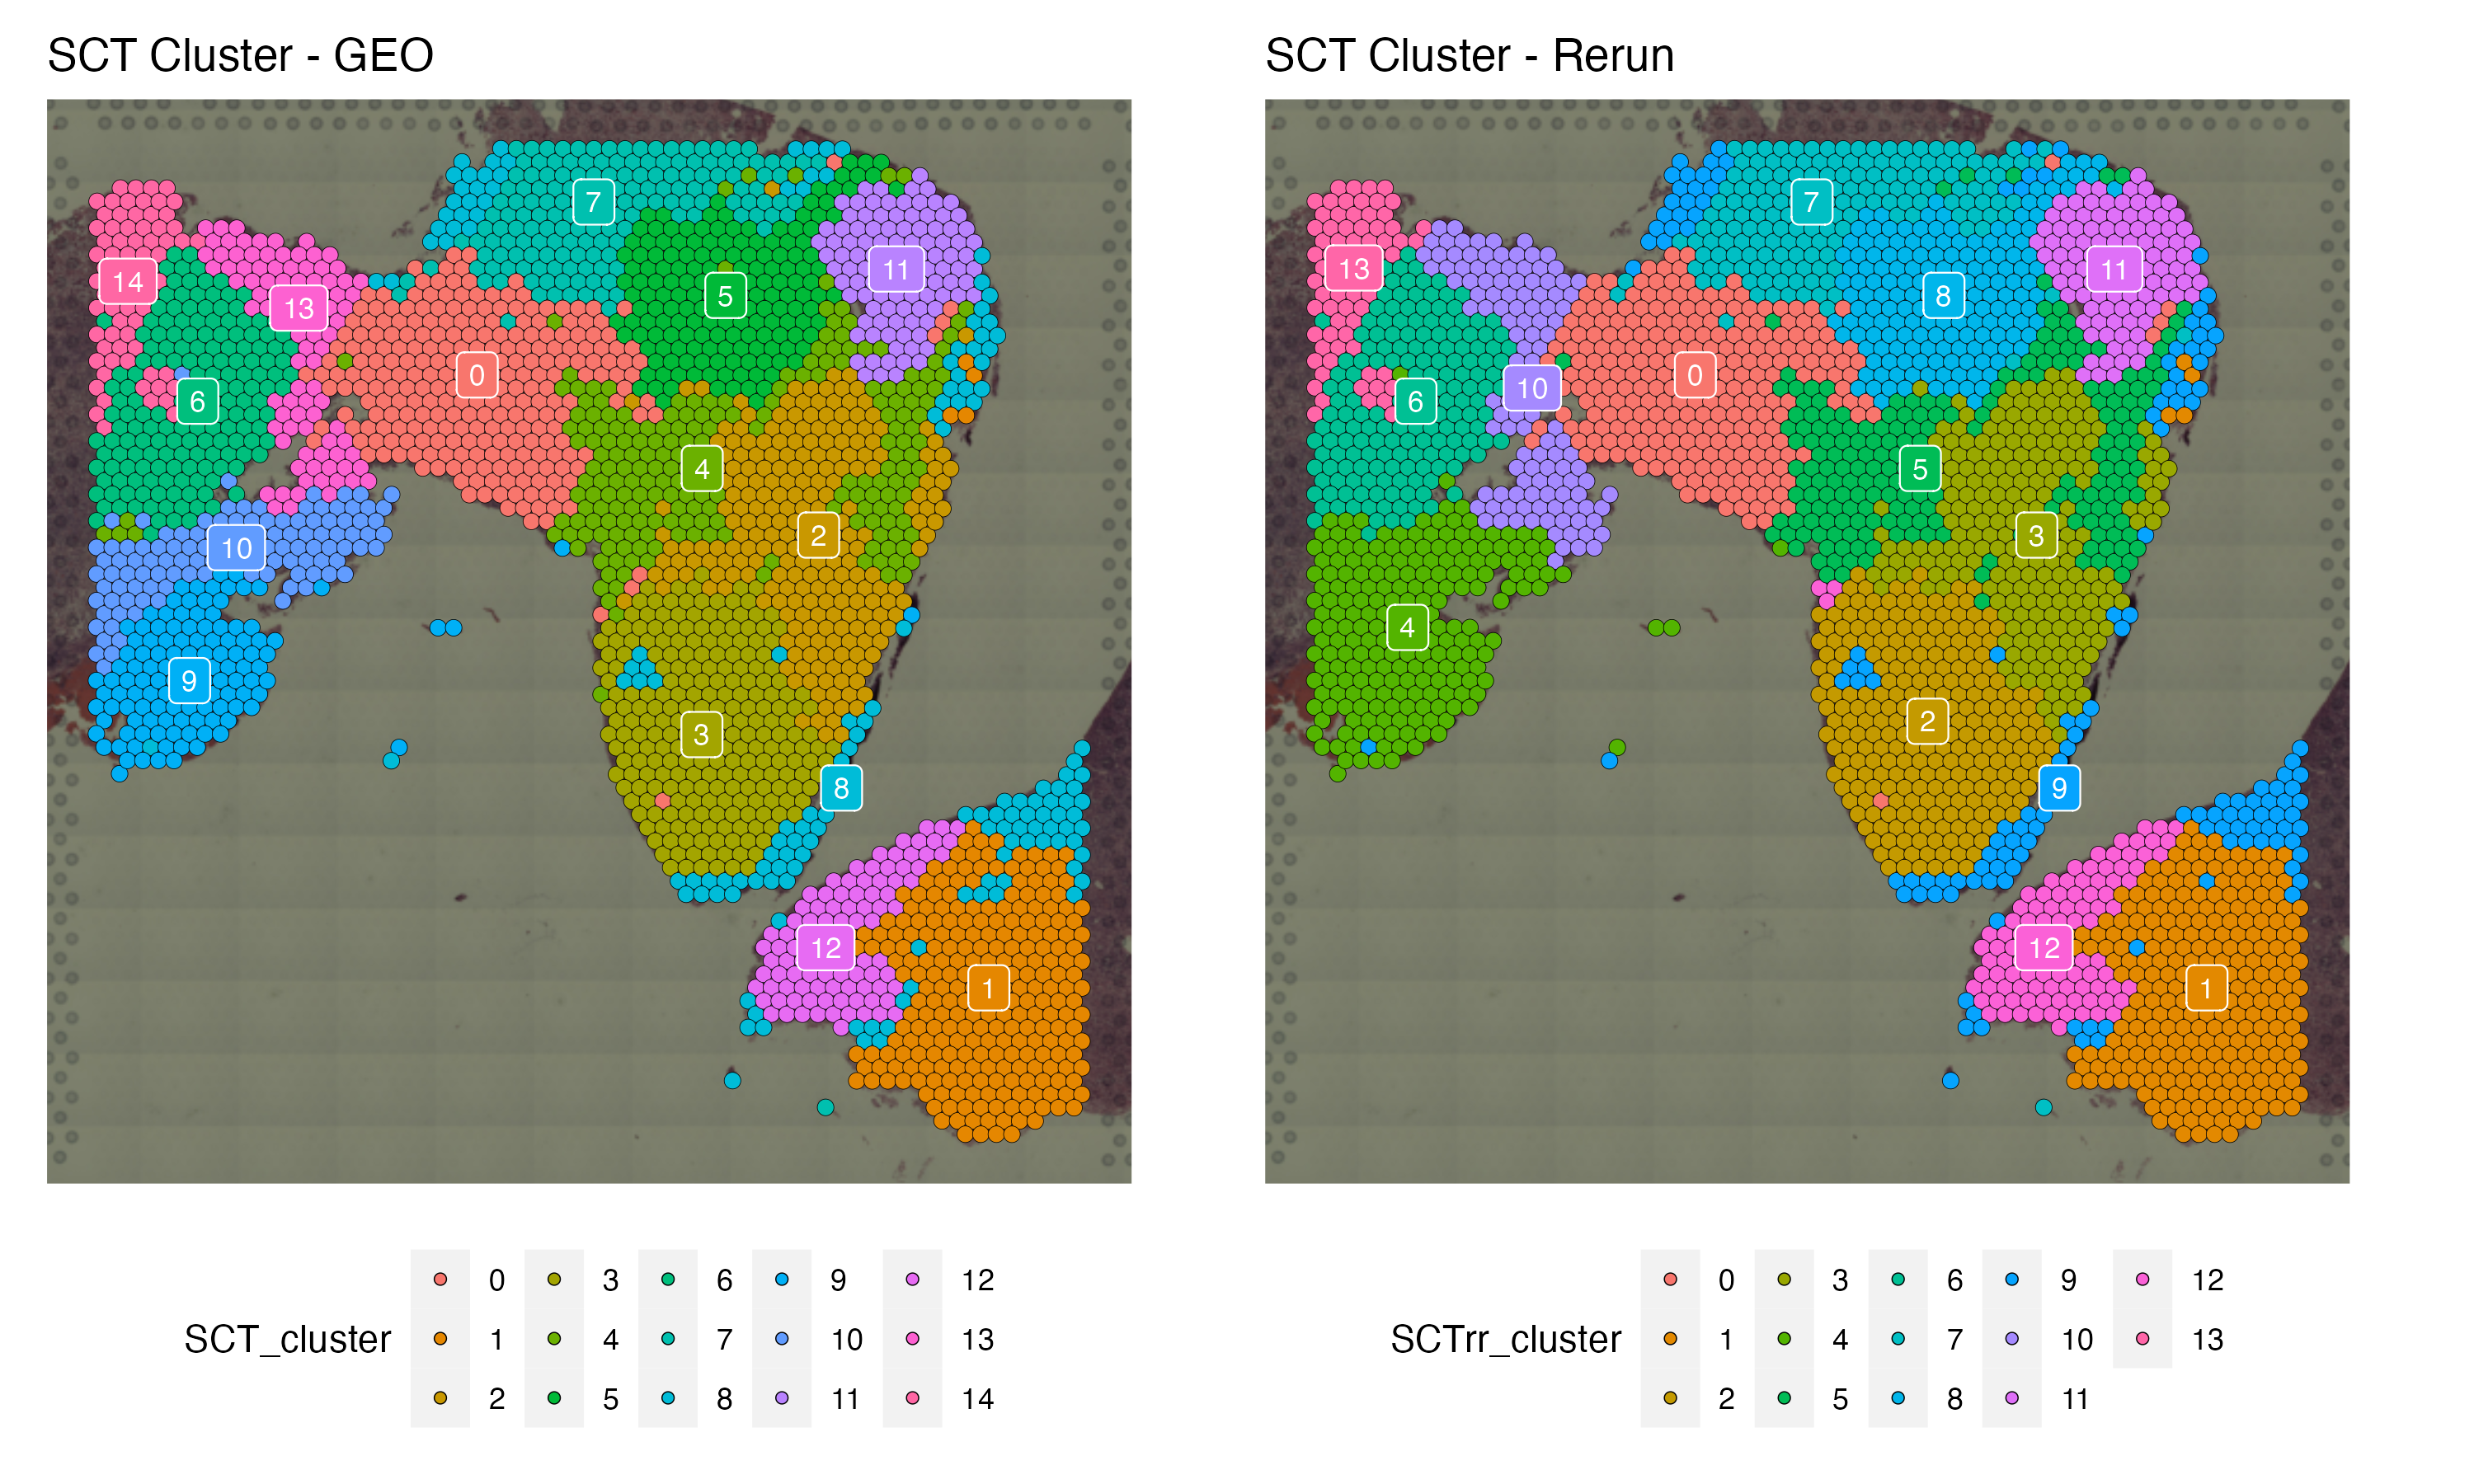
\includegraphics[width=\textwidth]{images/SpatialDimPlot_D_GTFB1170_SmallCellOvarianCancer_SCTrrcl.png}
    \caption{Replication of \citet{sanders_small_2022} SCTransform clusters, GEO metadata clustering on left and rerun clustering on right.}
    \label{fig:SCTcl_rr}
\end{figure}

\end{document}
